% !TeX root = ams_thesis.tex
\chapter{Related Work}

\section{Overview of Previous Swarm Hardware} \label{section:Overview_of_Previous_Swarm_Hardware}

Swarm robots are generally small. 
The reason to keep swarm robots small is related to both the cost of making them and the cost of using them. 
Larger robots consume more materials per unit, and so cost more money.
As a result, for a given number of swarm units, larger robots will result in a higher cost swarm. 
Also, each robot requires some amount of space to move around in. 
To keep the ratio of free space to robots constant, the area of space used by the robots grows as the robots do. 
If the ratio isn't kept constant, the robots will crowd each other, and so large robots will require either a very large space, or become overly crowded.
Finally, larger robots are more cumbersome to deal with. 
They require larger storage areas, possibly teamwork to lift or repair, and so forth. 
All of these efforts are also multiplied by the number of robots in the swarm. 
 
In addition to budgetary constraints, interaction with an environment built for humans places an upper bound the scale of the individual swarm members. 
For example, typical indoor doorways are around thirty inches wide, so a robot would have to be less than thirty inches wide to fit through them. 
The lower bound on swarm robots is generally dictated by fabrication technology, with smaller robots becoming increasingly difficult to assemble. 
As a result of these bounds, swarm robots are mostly between 1cm$^3$ and 0.3m$^3$. 
This scale range divides fairly evenly into robots that can operate in large swarms on a table, and those that can operate in swarms within a room, albeit possibly a large room. 
The challenge of construction of swarm robot hardware, then, is to put all of the same parts as non-swarm mobile robots: a mobility platform, a power supply, a processor, some sensors, and a communication system, into a small package.
Many impressive designs for small swarm robot platforms have been proposed and constructed as part of research in swarm robotics. 
However, most of these platforms are no longer easily commercially available, or never were. 

\subsection{Tabletop Swarms} \label{section:Tabletop_Swarms}

At the low end, in terms of size, the I-SWARM Project was intended to create a 2x2x1mm robot that moved by stick-slip locomotion actuated by piezo levers \citep{seyfried2005swarm}. 
Over the course of the project from 2004-2008, the hardware was developed and used in research, but was not converted to a commercial product.
Other techniques have been developed to use magnetic fields to apply force to small magnetic objects, resulting in controlled motion of the objects \citep{floyd2008untethered, pelrine2012diamagnetically}.
These systems are not amenable to decentralized control, because the moving components are not themselves robots. 
The moving parts are more accurately viewed as manipulators, with the instrumented environment, any sensors for feedback from that environment, and the manipulators themselves comprising a single robot. 

Early small-scale swarm robots were based on microprocessors, and were primarily research platforms for the groups that developed them, rather than commercially available products.
Alice, by Caprari \emph{et al}. combined a PIC16F84 processor, motors, RF and IR networking, and enough battery power for 10 hours of autonomy into a robot measuring under 2.5cm$^3$ \citep{caprari1998autonomous}. 
The Jasmine swarm robots were possibly the closest thing to a commercially-available successor to Alice \citep{kernbach2011swarmrobot}.
Jasmine measured 26x26x20mm, and included an ATMega processor, IR close range communication and obstacle detection, two motor skid steering, and lithium-polymer batteries.
Jasmine units cost about 100 Euro (\$111 USD) each when they were available, and they are no longer available for purchase. 
InsBot was a small robot, measuring 41mm x 30mm x 19mm, that was designed to interact with cockroaches \citep{colot2004insbot}.
It used two processors, one to run higher level behaviors and one to interface with a suite of sensors that included 12 IR sensors and a linear camera. 
The AmIR robot measured 6.5cm in diameter and 6cm tall. It has a more modern processor than Alice \citep{arvin2009development}.
There is no evidence that AmIR was ever widely available, and it cost \pounds65, or \$92 USD per unit \citep{arvin2015colias}.
The successors to Amir, Colias and the related Colias-$\Phi$, are dual-microprocessor systems similar to Jasmine in functionality, but with additional features for pheromone robotics applications \citep{arvin2014colias, arvin2015colias}. 
Colias is built out of two PCBs, with the upper PCB and processor handling IR collision avoidance and communication, and the lower processor controlling the motors, power management, and a few other sensors.
Colias robots cost \pounds25, or \$35US, in parts, but are not commercially available. 
The Colias-$\Phi$ model has an even more impressive price, at \pounds16, or \$22 USD.

Even when they are commercially available, most existing swarm robots are too expensive to build a large swarm.
The E-puck from EFPL is approximately 800 Swiss francs (\$810 USD) per unit, so the cost of maintaining a large swarm can become daunting quickly. 
The high price of the E-puck is a result of its extensive suite of sensors, including a camera and 360$^{\circ}$ IR range sensor and communication system. 

The r-one research robot is cheaper than the E-puck, at approximately \$220 USD per unit \citep{mclurkin2013low}. 
The developers of the r-one position it as a more featureful and less expensive alternative to the E-puck (\$810, cannot sense neighbors without additional hardware), Parallax's Scribbler (\$198, minimal sensors), the iRobot Create (\$220, requires additional hardware to be programmable), the K-team Khepera III (\$2000), and the Pololu 3pi (\$99, minimal sensors). 

The Harvard Kilobots are a more recent entry to inexpensive swarms, and have been produced in large quantities \citep{rubenstein2014kilobot}. 
Kilobots contain about \$15 worth of parts. 
However, this cost ignores the effort of assembling the robots. 
A 10-pack of assembled Kilobots sells for 1100 Swiss francs, or about \$112 (US) per robot. 
The Kilobots are intended for research in a highly homogeneous environment, with most or all of the robots executing the same program. 
As a result, they are designed to be programmed in parallel using an IR interface. 
For small groups, individual Kilobots can be programmed differently, but any attempt to give each of a very large collection of robots an unique program will take a long time. 
The Kilobots also move by stick-slip motion, and so must operate on a smooth surface, such as a whiteboard. 

The GRITSBots platform is a differential-drive platform using stepper motors \citep{pickem2015gritsbot}.
GRITSBots use the same processor as Colias, in a similar configuration, with one processor operating sensors and the other controlling the robot's motors. 
The sensor board incorporates a 3D accelerometer and gyro as well as a 6-direction IR distance sensing ring. 
GRITSBots measure 31mm x 33mm, and cost approximately \$50 for parts per unit. 

The Psi Swarm robot is a 10cm diameter round robot with proximity sensing, a compass, bluetooth wireless connectivity, and autonomous charging via ground contacts \citep{hilder2016psi}.
As with many of the platforms described in this section, it is not commercially available, but the designs to have the circuit boards fabricated and the body 3D printed are freely available. 

MROBerTO is a swarm robot with a 16mm$^2$ footprint. It has modular expandability via a header for daughterboards, and includes a single-point laser rangefinder, gyro, accelerometer, compass, and a VGA resolution camera \citep{Kim2016mROBerTOAM}. 
The mROBerTO processor is a 32-bit ARM processor with Bluetooth and ANT+ wireless. 
All of this hardware is only \$60 per unit in quantities of 25 or more units. 
In order to permit an overhead camera to localize the mROBerTO robots, a single RGB LED on top of the camera can be lit in a unique color to localize the robot, and a green LED on the front of the robot indicates its heading. 
The use of color information is likely much faster to process than fiducual tags, but does have the disadvantage that it is only useful in 2D unless a stereo camera is used. 

The Zooids of Le Goc \emph{et al.} are interesting in that the robots themselves are positioned as both a physical interface and a swarm \citep{le2016zooids}. 
They are designed to be used as physical controls, such as knobs or sliders, as well as being able to move themselves.
The individual robots measure 2.6cm in diameter, and localize themselves using a projected grey coded light signal from a high-speed projector. 
The authors estimate the individual cost of a Zooid at around \$50. 

Swarm robots have also been developed for aquatic and aerial robotics as well, although the problems unique to those domains are outside of the scope of this work \citep{costa2016design, preiss2017crazyswarm}. 
It is worth noting that the Crazyflie quadcopter platform on which the Crazyswarm is based is a commercial product, and so available to everyone. 
At least one legged, inexpensive robot platform has also been proposed as a swarm platform, but no swarm composed of them appears in the literature \citep{kalat2015tribot}. 

One way to reduce the cost of swarm robots is to use commercial, off-the-shelf (COTS) hardware in the construction of the robot. 
Reusing existing hardware leverages the economies of scale that reduce the price of commercial hardware, as well as eliminating the need to design or build the COTS parts. 
Use of COTS parts in research robotics has led to at least two platforms referred to as COTSBots \citep{bergbreiter2003cotsbots, soule2011cotsbots}.
The first COTSBots used mote hardware for the communications link and sensing, plus a motor control add-on board \citep{bergbreiter2003cotsbots}. 
The mobility platform is a modified toy, in particular, a specific brand of high-quality micro RC car.
At the time of this writing, the car used in COTSBots is moderately expensive for a toy car, although quite cheap for a research robot, costing a little over \$100USD per unit. 
COTSBots use TinyOS, a modular and event-driven framework for developing software for low-power wireless devices \citep{levis2005tinyos}. 


\subsection{Room-sized Swarms} \label{section:Room_sized_Swarms}

One potential problem with extremely small swarms is that while the robots may scale down, the obstacles they have to traverse do not scale with them. 
This sort of vulnerability prevents the smaller, tabletop swarm robots from operating well in human-scaled environments. 
In order to overcome this problem, larger swarm robots can be constructed.
 
The MarXbot swarm platform is capable of operating in unstructured human environments. 
MarXBots can also use their grippers to link themselves together and perform operations that an individual robot could not perform, such as bridging a gap larger than a single robot \citep{bonani2010marxbot}. 
The size and complexity of the MarXbots, as well as their powerful computer, renders the individual robots quite expensive. 

Swarmanoid extends the interlinking mechanism of MarXbot to a heterogeneous swarm with three different types of robots \citep{dorigo2013swarmanoid}.
The ``foot'' robots are MarXbots, and provide ground motion for ``hand'' robots. 
``Hand'' robots have grippers to manipulate objects, and can also climb.
The ``hand'' robots have an attachment point like the MarXbots, and so can be carried by ``foot'' robots. 
Flying ``eye'' robots provide overviews of the work area and networking.  

In order to reduce costs, another platform called COTSBots was developed \citep{soule2011cotsbots}.  
Instead of sensor motes on micro-scale RC cars, the newer COTSBots platform is composed of a laptop for processing and a modified RC car, tank, or similar toy as a mobility platform.
In order to interface between the laptop and motor drivers, a second micro-controller board, such as an Arduino or Phidget interface, may be used. 
Due to the diversity of possible combinations of hardware that can be assembled into this configuration, it is still a very viable platform. 
However, the minimum size of this style of COTSBot is the size of a laptop, which is in turn dictated largely by the minimum size of a useful keyboard. 
The large size of these COTSBots demands a very large space if the density of robots in a large swarm is to be kept low. 
Additionally, each laptop has a screen, keyboard, and so forth that are not useful while the robot is operating. 
All of these parts add to the overall cost of the swarm. 

Pheeno is an inexpensive robot of approximately the same scale as the MarxBots \citep{wilson2016pheeno}.
It has an optional gripper module, and uses a Raspberry Pi miniature computer for its main processing power. 
The developers of Pheeno provide a comparison with other robots in the same size range, which cost from \$150 for the Parallax Scribbler 2 to over \$3,000 for the much more sensor-rich Khephra IV. 

Beyond the scale of rooms, swarm research has been done with Amigobots and Roombas, as well as larger custom platforms for outdoor multi-robot work \citep{guo2007bio, tammet2008rfid, olson2013cacm}.
In theory, swarm research could be performed using robots of any size, but financial limitations would place it out of the reach of most academic organizations. 


\section{Swarm User Interface Designs} \label{section:Swarm_User_Interface_Designs}

The user interface to a swarm has two functions. 
The first is to allow the user to provide input to the swarm, so that the user can direct the swarm to perform tasks. 
For the purposes of this research, the user interface is a multitouch surface that displays representations of the area the swarm is in and of the individual swarm robots. 
The second function of a swarm user interface is to display information about the swarm, or to display information gathered by the swarm to the user. 
By providing an overview of the activities of the swarm, the user interface can give the user feedback on the progress of the task as it proceeds, as well as allowing the user to detect problems. 

Multitouch interfaces have been determined to improve on WIMP or voice interfaces for multi-robot control in a sequence of command and control tasks, including commanding the swarm to a location, performing reconnaissance, and having the swarm cross a dangerous area \citep{hayes2010multi}.
The interface displayed the locations of the robots on a directly manipulatable map, and used movable or semi-transparent user interface widgets, in order to minimize occlusion of the map. 
Areas were selected with with drawing gestures, and paths with fluid strokes, rather than e.g. selection of vertices bounding an area.
The use of multi-touch interaction is desirable because one-at-a-time selection doesn't scale beyond a very limited number of robots.
In order to interact with large groups of robots, the user must be able to perform operations on areas and groupings, rather than on the single point available with a traditional pointer-based interface. 

One approach to getting feedback from a swarm was the development of the Swarmish sound and light system \citep{mclurkin2006speaking}. 
Swarmish provides an ambient means of determining the overall state of the swarm, as well as some information about individual robots. 
The swarm that used Swarmish had autonomous charging, and so the individual robots had long runtimes, and minimal one-on-one interaction with humans. 
The ``ambient'' aspect of the interaction is that the information is continuously available, and the human user ``tunes in'' to it when needed. 
Swarmish uses a set of colored lights and sounds, produced by each robot, to provide feedback. 
The lights were in three colors, and had a total of 108 different combinations of colors and blink sequences, as a visual indicator of the state of each robot. 
In addition to the lights, each robot could produce MIDI notes over its audio system. 
Each note could vary in instrument, pitch, duration, and volume, as well as having tempos and rhythms as the code executes. 
The designers of Swarmish indicate that the sum of the audio output of the swarm could provide a overall idea of the status of the swarm, but that as a musical instrument, it is difficult to play well. 
Further, the use of lights as signaling mechanisms assumes that you can look at the robots. 

If we accept the assumption that the robots are visible to the user, the robots can carry some form of display that provides local information to the user. 
This information can then be displayed as an overlay in the real world, with the display of the information conterminous with its presence \citep{Daily:2003:WEI:820752.821587}. 
For example, if each robot has a gas sensor, and a light that it can illuminate in response to detected gas, then the user can look at the swarm, and see which areas of the swarm are detecting gas.
Local display of local information works if the user is part of a hybrid human/robot team, and so is in the same location as the users. 
However, there are many situations where the robot is not in the same location as the user. 
A common example is urban search and rescue, where buildings may be known to be unsafe, or of unknown stability, but it is desirable to search them for trapped people. 
In such a situation, the human user would rather be located elsewhere, and receive information from the robots. 

For situations where the user is not located in the same area as the robots, one possible approach is a ``call center'', where robots can request human attention when required \citep{chen2011supervisory}. 
The human in the call center, however, is faced with having to answer potentially multiple calls with no awareness of the robot's situation. 
The theoretical basis for call center UI is Supervisory Control. 
Supervisory control has the human act as the planner and monitor of the systems being supervised, but allowing the systems to operate on their own.
Automation is frequently broken down into ten levels of automation, with level ten being a fully automatic system with no humans involved, and level one having no automation, such as a bicycle \citep{parasuraman2000model}. 

It would be expected that reducing the number of times the human is required to interact with the robot will permit the user to operate more robots.
With level one automation, the user has to interact constantly, and so could not be expected to operate more than one robot. 
By increasing the level of autonomy of the robot, the time required for the user to operate the robot decreases.
Instead of continuous interaction, the user can specify actions for the robot to undertake, and then ignore the robot while it performs the actions.
It is expected that the robot's effectiveness will decline over time since the last user interaction. 
This time that the robot operates without interaction before its effectiveness declines to a fixed minimum is called ``neglect time"\citep{olsen2003metrics}.
With increasing autonomy, neglect time increases.
The fifth level of the autonomy scale is operation by consent, where the computer chooses a route and executes it if the human permits it. 
The ninth level is the inverse of the fifth.
Rather than asking the user for consent to act, the robot acts autonomously and informs the human only in exceptional cases.
At the higher levels of the autonomy scale, the robot's neglect time far outweighs the time the user is expected to operate it, and so the user could reasonably be expected to operate other robots during the neglect time. 

Increasing neglect time may allow the user to operate more swarm robots, but it comes at a cost. 
The longer a user goes without learning about the state of one of the robots, the less idea they will have of the robot's situation when they are called upon to operate that robot. 
The problem of automation decreasing the situational awareness (SA) of the user has been described in cockpit automation for aircraft \citep{wiener1980flight}, and generalized well to other systems that combine automation with human control \citep{kaber1997out}. 
If the user takes a long time to relearn the situation, the efficiency of the system will drop. 
Worse, the user may make errors because of an incorrect understanding of the system when they begin operations after a long neglect time \citep{cummings2008predicting}. 
One possible approach to maintain a constant and manageable workload on the user is adapting the level of automation to the workload. 
When the load is low, the user is more directly engaged, but when load is high, there is more automated assistance. 
By varying the level of automation, the workload for the user is kept constant. 
A constant workload is desirable because the user remains engaged with the work, and so has an ongoing understanding of the situation as it develops. 
The user is not suddenly called into a situation after remaining disengaged for some time. 
However, the workload must also be manageable. 
If the user is overloaded, their attention will become subject to triage, and they will begin to miss elements of the task. 
Adaptation does not have to be based on measured load, but could instead be based on perceived load or physiological markers in the user. 
%\citep{goodrich2010maximizing}

However, in situations with even moderate numbers of robots, even relatively high levels of automation may overwhelm the user \citep{lewis200617}. 
Level five, operation by consent, is a fairly high level of autonomy, but with a large number of robots checking in, even this level may generate too many events for the human to deal with. 
Increasing the autonomy to level nine, so that the robots are only checking in with the operator when an exceptional situation occurs, may still overwhelm the operator if enough robots are active.
Increasing the use of automation may also create new difficulties by leaving operator out of practice, or encouraging mis-placed trust in the automation's ability \citep{lee2004trust}. 

In fact, any kind of multitasking may prove insufficient for large swarms. 
For teleoperation, the best case is uncrewed aerial vehicles (UAVs), which require relatively little oversight. 
Uncrewed ground vehicles (UGVs) require more oversight than UAVs, due to the higher complexity of the ground environment. 
Estimates place the limits on the number of robots under control at 12 or 13 for UAVs and 3-9 for UGVs \citep{WangSearchScale}.  
There is some latitude, at least in UGVs, to increase multitasking by increasing automation, as shown by the relatively wide range in the interaction limits, but even 9 robots per operator is nowhere near the scale of kilo-robot swarms  \citep{Olsen:2004:FMH:985692.985722}.
Failure generally takes the form of task effectiveness no longer increasing as more robots are added.
Instead, the amount of time the user spends interacting with the robots begins to outweigh the neglect time, and so the robots spend increasing amounts of time waiting for interactions \citep{cummings2008predicting}. 

Ecological interface design (EID) presents a possible guide to the architecture of user interfaces for swarm robotics, and has been used in interfaces with mixed human-robot teams \citep{vicente1992ecological, gancet2010user}. 
In EID, a user's abilities that enable them to interact with a system is separated into a taxonomy of skills, rules, and knowledge. 
The user has skills, which are rote, simple activities that form the basis of the normal operation of the system. 
The user also knows a set of rules about the system. 
Rules allow the user to handle exceptions or unusual cases that have come up before. 
Rules do not require the user to understand the system, just to know that when certain situations are recognized, certain actions must be performed in response. 
Beyond rules and skills, the user also has knowledge of the system. 
Knowledge gives the user an understanding of how the system works, which they can apply to react to situations that the user has not experienced or been told about before. 
Events are also broken into three levels: routine, which uses skills; foreseen exceptions, which use rules; and unforeseen exceptions, which use knowledge. 
All levels should be supported by the interface, but the user should not be forced to operate at a higher level than is required. 
The abstraction of the process maps onto the hierarchy of ecological design, with the highest level being the function of the process and the lowest level being how the function is accomplished. 
At each level, there are constraints on the process that are used to define the normal operation of the process.
Detection of exceptions requires the display of all constraints, because exception is the breaking of constraints, and undisplayed constraints cannot be assessed to determine if they have been broken.

The user should be able to extract meaning from the information display quickly, as in the case of Swarmish and the robot-as-pixel UI designs.
By using the lights in Swarmish, the user can assess the state of individual robots, but by listening to the overall sound of the swarm, the user can also assess the behavior of the system as a whole.
The state and status lights of an individual robot is the low level in EID, watching how an individual action of the overall process is progressing. 
The ``tune'' of the entire swarm, produced by the sum of their MIDI notes, provides the high level overview, where a user can tell if the system is progressing well or developing problems. 
As the system changes, the changes and predictions should be highlighted so that the user understands consequences of their actions. 
In Swarmish, sudden changes in the tone or tempo of the swarm tune indicate transitions in its behavior, without the user having to observe the actions of the robots closely. 

EID is well-positioned to deal with emergent behavior, because the emergent behavior of the entire system is present at the functional level, but is composed of actions at the physical level.  
The control of swarm robots can be viewed as a hierarchy of increasing abstraction. 
At the least abstract, base level are the individual interactions of the swarm robots with each other and their environment, as dictated by their explicit programs. 
Above that level is the implicit, emergent behavior of the swarm as a whole. 
Finally, the most abstract level is the user intent, as expressed in the interface through their gestures. 
This hierarchy corresponds well to the abstraction of process in EID, with discrete physical actions at the lowest level and the overall results of the process at the highest level. 
Consequently, the user is permitted to issue commands in the most abstract domain, and the system can propagate them ``downwards'' into the concrete actions of the robots in the world, while also propagating information from individual robots ``upwards'' into the global view. 

Automation in EID allows the user to operate primarily with rules and knowledge, dealing with exceptions \citep{vicente2002ecological}.
The interface should allow direct manipulation of perceptual forms that map directly onto work-domain constraints and represent all of the information identified by the abstraction hierarchy. 
In a swarm context, this means displaying functional information in such a way that the user can move across the hierarchy from individual swarm robots to high-level swarm-wide tasks, and interact at all levels to control the swarm. 
More practically, this means that the information displayed must be integrated in such a way that the mapping from one unit of information to another is made apparent in the interface, rather than offloaded to the user to compute in their head \citep{yanco2004beyond}. 
For example, if a robot can send video and range information, the information can be projected into a 3D space around the robot, rather than being displayed in separate UI windows.
Such a projection allows the user to easily relate visual and range information, and relate that information to the ongoing robot control task, which in turn increases task performance \citep{ricks2004ecological}.
Previous work in multi-touch interfaces directly satisfies these requirements of EID by providing both an omniscient camera view for direct manipulation of the high-level, functional actions of the entire swarm, and the ability to move down the hierarchy to control individual swarm members \citep{Micire:2009:ANG:1731903.1731912}.
The ability to display information about individual robots along side or on top of the interface representation of the robot is an important method of providing feedback to the user \citep{Kato:2009:MIC:1520340.1520500}. 

Due to their strategic potential, research in human-swarm interface for UAV swarms is a rapidly developing field \citep{hocraffer2017meta}. 
Potential issues for an interface can be cognitive limitations of the users, or actual design problems in the interface. 
Research in the field attempts to measure the difficulty of using the interfaces in a number of ways, including cognitive workload, task effectiveness, effective use of operator time, and situational awareness. 
Perhaps due to the expected mission parameters, very few studies are performed using swarms of more than tens of robots. 
%\todo{more write up of this paper, follow it's cites}

Because of the limitations on individual sensing, especially in the case of a robot with poor localization, providing a third-person user interface rather than a first-person one is better for control of swarm robots \citep{kapellmann2016human}. 
Kapellmann \emph{et al.} provided a user interface that allowed users to control swarms through the influence of teleoperated leaders. 
Because teleoperation places the user in the point of view of the individual robot being operated (as with many combat UAV interfaces), the user had some difficulty acquiring an idea of the overall disposition of the robots. 
Once the user was provided with a third-person, ``eye in the sky'' view, their performance increased. 
Users with global information were able to aggregate 90\% of the robots, as opposed to approximately 50\% in situations without global information. 

\subsection{UI Designs}
Previous work in multitouch user interface gesture sets can be broadly separated into two classes: those that attempt to build a general gesture set, and those that attempt to build a gesture set to be used for a specific task. 

General gesture sets would be for operations such as the cut/copy/paste editing metaphors, which show up in word processing, image editing, and other productivity applications. 
These operations act in in differing ways, depending on their context, but are conceptually similar, e.g. paste always inserts information that was previously cut, but the information type may vary. The operations are also invoked in the same way across applications and even across operating systems. 

Wobbrock, Morris, and Wilson use an interesting technique to elicit general user-interface gestures from non-technical users \citep{wobbrock2009user}.
The user is shown the \textit{effect} of a command, and then asked to perform the gesture that \textit{caused} that effect. 
The users were asked to think aloud, in order to understand their cognition about the system and gestures, in addition to their behaviour. 
The experiment used 27 commands: move a little, move a lot, select single, rotate, shrink, delete, enlarge, pan, close, zoom in, zoom out, select group, open, duplicate, previous, next, insert, maximize, paste, minimize, cut, accept, reject, access menu, help, task switch, and undo (listed in order of complexity as ranked by Wobbrock \textit{et al}).
Many of these commands are related to window managers, or occur in some form in multiple applications, such as the cut/copy/paste metaphors.

Task-specific gestures are for operations such as flying through a 3D rendering of an architectural space, or transposing cells in a spreadsheet. 
While somewhat intuitive gestures may exist for both operations, the operation is tightly bound to the task at hand, and the gestures would likely be different. 

Yao, Fernando, and Wang develop a set of task-specific gestures for urban planning from the required functionality of the interface and paper prototyping on a table \citep{yao2012multi}. 
The gestures were collected by placing a map on the table, and asking users to perform the gestures they would use to access the required functions. 
The resulting interface is modal.
Depending on the selected mode, different gestures are available. 
The interface also permits the combination of some gestures, such as panning or rotating the map while zooming in or out at the same time. 

Micire \textit{et al}. developed a taxonomy of user gestures for control of both robots and of the interface to control them \citep{Micire:2009:ANG:1731903.1731912}. 
The interface control gestures are for actions such as zooming in on the content of the screen or panning around a map. 
Individual users chose a variety of gestures to perform the tasks, but for almost all types of tasks, having two gestures available to perform it would be sufficient to cover 60\% of the users. 
It was also noted that the gestures that users use are informed by their previous experience both with traditional mouse-oriented windowing interfaces and with touch-screen technology. 
Since smartphones are a common multitouch interaction device, it would be expected that smartphone users expectations of multitouch interaction would be informed by their phones. 
Micire \textit{et al}. confirmed this, finding that iPhone owners used significantly more pinch gestures than participants with no iPhone experience. 

The more general gestures sets, such as those from Wobbrock, Morris, and Wilson, could be used in a gestural window manager or operating system interface. 
They are not tied to a specific application or working with a specific type or presentation of data.
The gesture sets developed by Micire \textit{et al}; Yao, Fernando, and Wang; or in this work, are all intended to provide a more precise set of meanings for a single application and task. 


\subsection{Multitouch UI Design Concerns} \label{section:Multitouch_UI_Design_Concerns}
Multitouch user interfaces do not have an agreed-upon standard for the gestures used in interaction with them, largely due to the relative novelty of the technology. 
Early in the development of multitouch user interfaces, it became apparent that the window, icon, menu, and pointer (WIMP) interface would not be the best way to interact with novel interface technologies \citep{van1997post}. 
WIMP interfaces are tied to a metaphor of a desktop, where a user interacts with 2D spreadsheets and documents. 
To extend to information with higher dimensionality, the interfaces become more complex and less direct. 
The somewhat precient model proposed in by van Dam is a multi-modal interface of gestures and natural language, as is found in modern smartphones. 
This paper also shows an early example of a two-handed manipulation of a virtual object in a 3D environment, which presages the direct interaction style of multitouch user interfaces. 

The directness of user interactions can be understood to be the degree to which the interaction resembles the same interaction with physical objects, such as flipping pages of a calendar. 
With a physical calendar, one can turn pages by sliding a finger over them. 
Having a slider or buttons to switch months in a virtual calendar is thus less direct, and with a mulitouch interface, can be replaced by the same finger motion that would flip a page of a physical calendar.

This sort of emulation of design elements of an object the same when the object is moved to a new material or created by new techniques is called ``skeueomorphism", and the copied design elements are ``skeueomorphs''. 
There are several reasons for skeueomorphs in design of user interactions. 
One reason is effectively kitsch. 
Design elements can be kept, despite not having a function in the new medium, simply because people find it entertaining to keep the appearance.
The vestigial jug handles on bottles of maple syrup or the yellow ``paper'' background of Apple Notes prior to its redesign are an example of this type of skueomorphism.
The jug handles are too small to use as handles, and the ``paper'' of Apple notes has no effect on the functioning of the application. 

Another reason to keep a design element, especially in multitouch UIs, is that the design element may provide hints to the user as to how the object can be interacted with. 
For example, in displaying photos, if the photo has a slight border, and the border appears to curve and ``lift'' off the screen background slightly, it will imply that the photo is a mobile object with a small space under it, and so could have other photos under or on top of it. 
If the photo is displayed totally flat, without a border, it will look more like a sticker or part of the background, and not imply that it can be moved. 
In neither case is the image actually ``above'' the background, but the visual impression to the user provides a clue for interacting with it. 
The interface itself can be viewed as a message from the developer to the end user, which hopefully conveys enough information about the design of the interface to the end user that they are able to use it \citep{derboven2012semiotic}. 

In the study of interactions with tangible interfaces, it has been proposed that the use of skueomorphic interfaces can also bridge between these two reasons for their use \citep{gross2014skeu}.
Rather than simple functionality, or pure amusement, the use of skueomorphic interface designs can convey messages about abstract qualities of a product to a user. 
One example given by Gross, Bardzell, and Bardzell is a digital synthesizer with a user interface that copies the knobs and switches of physical analog synthesizers. 
While this is likely not an optimal interface for controlling the synthesizer, it has connotations of quality, performance, and reference to more traditional electronic instruments, and so appeals to the user's idea of themselves as an artist and a participant in a tradition of artists. 

\subsection{Human/Swarm Interaction} \label{section:Existing_Research_on_Swarm_Controlability}

There does not appear to be a consensus on how the user interface for a swarm should work
Indeed, the term "Swarm UI" is sometimes used to describe the user interface to a swarm, and sometimes used to describe a user interface which is itself a swarm \citep{le2016zooids, suzuki2018reactile}

Swarm interaction is distinct from multi-robot HRI. 
Multi-robot HRI interfaces typically allow the user direct control of individual robots, which can be switched betweenm but generally do not treat the group as a whole. 
An example of a multi-robot HRI study is the assessment by Humphrey et al of the scalability of a multiple-robot control interface that uses a ``halo'' around the view from the currently-controlled robot to provide awareness of the positions of the other robots \citep{humphrey2007assessing}
While this interface did appear to have a positive influence on the number of robots the user could control, it is not a swarm interface, but an interface for individual control of multiple robots. 

Previous work in human-swarm interaction (HSI) shows an interesting diversity of methods to convey a command to a swarm. 
One approach, for co-located swarms, has the user making hand signals to the robots. 
If the swarm is equipped with cameras, the hand signs can be recognized visually by members of the swarm \citep{nagi2014online, giusti2012human, nagi2014human}. 
Because the recognition is performed by multiple robots at once, with different views, the robots can confer among themselves to arrive at a better understanding of the sign used.
Another approach to gesture control of swarms is to have the human and gesture recognition hardware separate from the swarm \citep{alonso2015gesture}.
This approach also allows the software to use the user's gestures to select part of the swarm by natural methods, such as pointing at robots. 

Another approach is the management of attractive and repulsive forces in the interface, which are conveyed to the robots. 
This style of interface maps reasonably directly to at least three of the programming paradigms used in swarm robotics. 
In physicomimetics, the attractors or repellents are points in the field that act on the robots through the same forces that the robots use in their interaction with each other. 
To cause robots to gather in an area, the user could place a source of virtual gravity there, which would draw robots towards it. 
In pheromone robotics, the effect would be much the same, but would be expressed as a pheromone source that diffused into the space and attracted robots. 
In vector fields, the vector field itself would be changed so that all vectors pointed towards the desired location. 
One implementation of a human-swarm allows the human operator to describe the desired density of robots at locations within an operating area \citep{diaz2017human}. 
The use of density, rather than robot count, scales with the swarm size.
The desired configuration of the swarm can be drawn by the user on a tablet, and then converted to an update control law for the robots.
Alternatively, the user can directly place Gaussian functions in the space and vary their parameters. 
The resulting desired densities are smoothed to avoid discontinuities.

The use of density over location is similar to a number of interface methods that function by allowing the user to specify attractors and repulsion points in the swarm space \citep{goodrich2011toward, brown2014human, vasile2011integrating, kira2009exerting}. 
Goodrich et al use an attractor model under two different design metaphors, physicomimetics and a biomemetic model based on the dynamics of schooling fish, to solve an abstract information foraging problem \citep{goodrich2011toward}. 
The human influence is applied to a swarm system that is capable of some aspects of the problem without supervision, but is improved by the addition of human control. 
In keeping with the bio-inspired metaphor, the human can either control a leader, which the other members of the swarm are attracted to and follow, or a predator, which repels and can chase other members of the swarm. 
Leader-based models tend to lead to more stable, long-running interactions, as the members of the swarm move to remain near the leader, increasing the duration of the human operator's influence on the leader. 
In contrast, predator models result in high turnover of the swarm members that the human can influence, as the ``prey'' elements of the swarm act to get away from the predator's influence. 
This turnover is part of the two invariants proposed for swarm interaction by Brown et al, which are that the collective state is the fundemental perception of the swarm, rather than the individual robot, and that the ability of a person to influence and understand the collective state is determined by the balance between span and persistence \citep{brown2015two}. 
Persistence is the duration of each interaction with the swarm, and span is how many units the user interacts with. 
In a leader-based control UI, the span and persistence are both kept high, because the swarm elements are attracted towards the leader and remain under its influence for longer. 
In the predatory/repellent model, the span and persistence are low, because the other swarm elements flee from the user-controlled predatory unit. 

Brown, Kerman, and Goodrich demonstrate that a swarm can be controlled to form two different higher-level structures, a flock and a torus, by managing abstract attractors rather than individual behaviors. 
Further, the transition between modes was amenable to human control, so the overall behavior of the swarm could be configured with a relatively small set of tunable parameters. 
While the paper only indicates two possible modes, the torus and flock, these two behaviors are a relatively good match for the publicized behavior of the Perdix military drone swarm. 
Flock is a useful behavior for organized motion to a location, while the torus mode is good for loitering and overwatch of an area, matching the point-orbit, and move-to-point functions that are visible in videos of the Perdix UI. 
However, public materials on the Perdix system indicate that it uses a playbook interface, where the user selects from a set of available ``plays'', which the swarm then executes, rather than an explicit management of attractor parameters \citep{PerdixFactsheet}. 

Parasuraman, Galster, and Miller examined the use of playbook, waypoint, and combined playbook and waypoint control on robot teams in a capture-the-flag task \citep{parasuraman2005flexible}.
Playbook control provides a delegation layer to the interface, where the user does not have to specify the minutia of how a task is completed. 
The use of delegation decreases mission time and increases success, in this case, winning the game of capture-the-flag.

There have been previous studies of the behavior of users in control of swarms with poor localization and bandwidth constraints \citep{nunnally2012human}. 
These constraints are realistic, as the motivating examples for swarm robotics, such as urban search and rescue or planetary exploration on e.g. Mars take place in locations where high-speed and high bandwidth networking infrastructure may be absent. 
The study describes a task similar to foraging, but under human control, where a 30-robot swarm is used to find a sequence of targets. 
The interface is mouse-based, and allows the user to issue two commands, "head towards the selected point" and "stop". 
The robots had gaussian error added their estimated location and orientation, meaning that the robots could start on a heading that was not exactly towards the selected point, when the user gave them a point to move towards. 
However, the robots had a consensus algorithm that would allow them to match heading with neighbors, which acts to counter the error in their initial headings. 
There were three conditions: low swarm-to-swarm bandwidth with low swarm-to-user bandwidth, high swarm-to-swarm with low swarm to user bandwidth, and high swarm-to-swarm bandwidth with high swarm-to user bandwidth.
The results showed that the medium bandwidth condition, with high swarm-to-swarm bandwidth but low swarm-to-user bandwidth was sufficient to complete the task. 
The users did adapt their behavior to match the information they had available, issuing more commands closer together in the medium bandwidth condition to drive the swarm into a smaller region and increase intra-swarm connectivity. 
In the low bandwidth condition, the user did not receive updates about the swarm condition often enough to enable them to maintain a dense swarm, and as a result, had trouble finding targets. 
The fact that the user interface and the user's intuition about the swarm could drive adoption of different behaviors supports the use of different rendering schemes for the swarm to encourage different user control strategies or conceptualizations about the swarm. 

Nunnally \emph{et al} explored the condition where a limited amount of information was available, but the time it takes for that information to become available (latency) is another factor in human-swarm interaction \citep{walker2012neglect}.
In the study , the latency was either absent, present both between members of the swarm and between the swarm and the user, and present, but the interface to the user predicted future swarm motion and displayed it. 
The task was similar to Nunnally \emph{et al}, in that the swarm was used to search a region for targets in a foraging task. 
The swarm could be commanded to move to a heading, stop, or flock under a model similar to boids \citep{reynolds1987flocks}.
The latency condition was significantly worse, in terms of targets found, than the no-latency condition, but the predictive display countered the latency sufficiently that the predictive and no-latency conditions were not significantly different. 
Interestingly, latency also drove the appearance of what the authors refer to as ``neglect benevolence", where the user not interacting with the system was not only tolerated, but actually helped improve the behavior of the system. 
Under latency, the user would issue a command, and then wait out the latency period to see how the system responded.
The resulting delay allowed operations such as flocking to converge and stabilize, thus increasing the swarm connectivity beyond what was attained in the no-latency condition. 

The previously discussed work on attractor management and control under latency and bandwidth restriction is concerned with UI design for swarm robots from the point of view of controllability and influence, which is to say whether or not the user can maintain desirable aspects of the swarm under the given conditions. 
It is not largely concerned with whether the interface itself, as presented in the experiment, is the best way for the user to attempt to control the swarm.
That is to say, the interface is taken as a fixed point, and the experimental condition is variation in the quality of the link between the user interface and the swarm. 

Kolling et al compared two forms of influence-oriented UI, selection and beacon based control, with a variable number of robots \citep{kolling2013human}. 
Selection control requires that the user select groups and then influence the selected group or put them into a specific autonomous behavior mode. 
This is arguably a form of playbook control, where some robots are selected and then given a play to execute. 
Beacon control has the user place beacons that attract the robots with a range, which is form of leader or attractor-based control. 
The paper also divides these control methods into intermittent, for selection, and environmental, for beacons. 
The intermittent method is called that because the user issues infrequent commands, rather than continuously operating the group. 
This is in opposition to a persistent control method, where the user might directly operate some of the robots with a joystick or other constant control input, as in some predator/leader systems. 
The beacons are environmental, because rather than interacting with the robots, the user interacts with the beacons and their locations in the environment. 
Selection control outperformed beacon control, especially as the number of robots in the swarm increased. 
The authors indicate that as the swarm size increased, the per-robot precision of beacon control decreased, while selection control remained constant, allowing the user to exert a more precise influence over the swarm. 
This indicates that the selection and operation control scheme used in this thesis is a better method for controlling large swarms than beacon or attractor based schemes. 
However, humans were solidly outperformed by fully autonomous benchmarks developed to more optimally perform the foraging task in the experiment, which indicates that human control is more useful in conditions where the humans may have access to information that the robots do not have access to. 
Otherwise, human control may present a bottleneck, rather than an advantage. 

\subsection{The Interfaceless Interface} \label{section:The_Interfaceless_Interface}

Some swarm robots are designed to be used with no control interface at all.
By altering the shape of simple stick-slip locomotion toys with laser-cut foam ``hats'' that change their outer perimeter, and changing the outline of the laser-cut foam forms they interact with, the random motion of the toys can create stable structures \citep{andreen2016emergent}).
The development of the shapes relies on human interaction, but specifying the shapes of the hats and interactive components seems amenable to solution with genetic algorithms. 
Because the toys used in this work were about \$4-8 USD, and everything else was composed of laser-cut foam, the platform is extremely inexpensive, but the tasks it can solve are seemingly limited to self-assembly. 

The Guardians project studied the deployment of sensor-equipped robots to support firefighters by providing mapping and sensor information that would not normally be available to the firefighter \citep{gancet2010user}.
Rather than having the firefighter control the robots, the robots would deploy with the firefighters and swarm with them, attempting to maintain network connectivity and proximity to the firefighter. 
The robots provide a stream of information via a heads-up display (HUD) constructed of LEDs on the firefighter's visor, which the firefighter may or may not choose to react to. 
Instead of having to control the swarm, the user acts as they feel is best, using both their own information and that from the swarm of robots that surrounds them and extends the firefighter's senses \citep{penders2011robot}. 


\subsection{Video Game UI Design} \label{section:Video_Game_UI_Design}

There is a general resemblence between many of the overhead-view interfaces for swarm robot control and the interfaces used in video games for control of multiple units, especially in the genres of Real Time Strategy (RTS) games, Turn-based strategy games, and Multiplayer Online Battle Arena (MOBA). 
Interestingly, most multi-unit video games UIs operate using a selection, rather than beacon, interfaces, according to the classification of interaction methods by Kolling et al. 
The influence of user interaction affordances in games with overhead views and control of multiple units may be a rich area of study for researchers in human-robot interaction, and especially human-swarm interaction. 
Previous work in group robot control has indicated that user experience with video games influences the interaction methods that they would like in a user interface \cite{micire2010multi}.
Users who play video games express a desire for more UI ``widget'' interactions, that is, interacting with buttons, menus, or specialized user interface components \cite{Micire:2009:ANG:1731903.1731912}. 
Gamers who play Real Time Strategy (RTS) games also used fewer pinch gestures in a multitouch context, possibly because RTS games are typically played with a mouse and keyboard, which does not have a pinch-like gesture. 

\begin{figure}
	\centering
	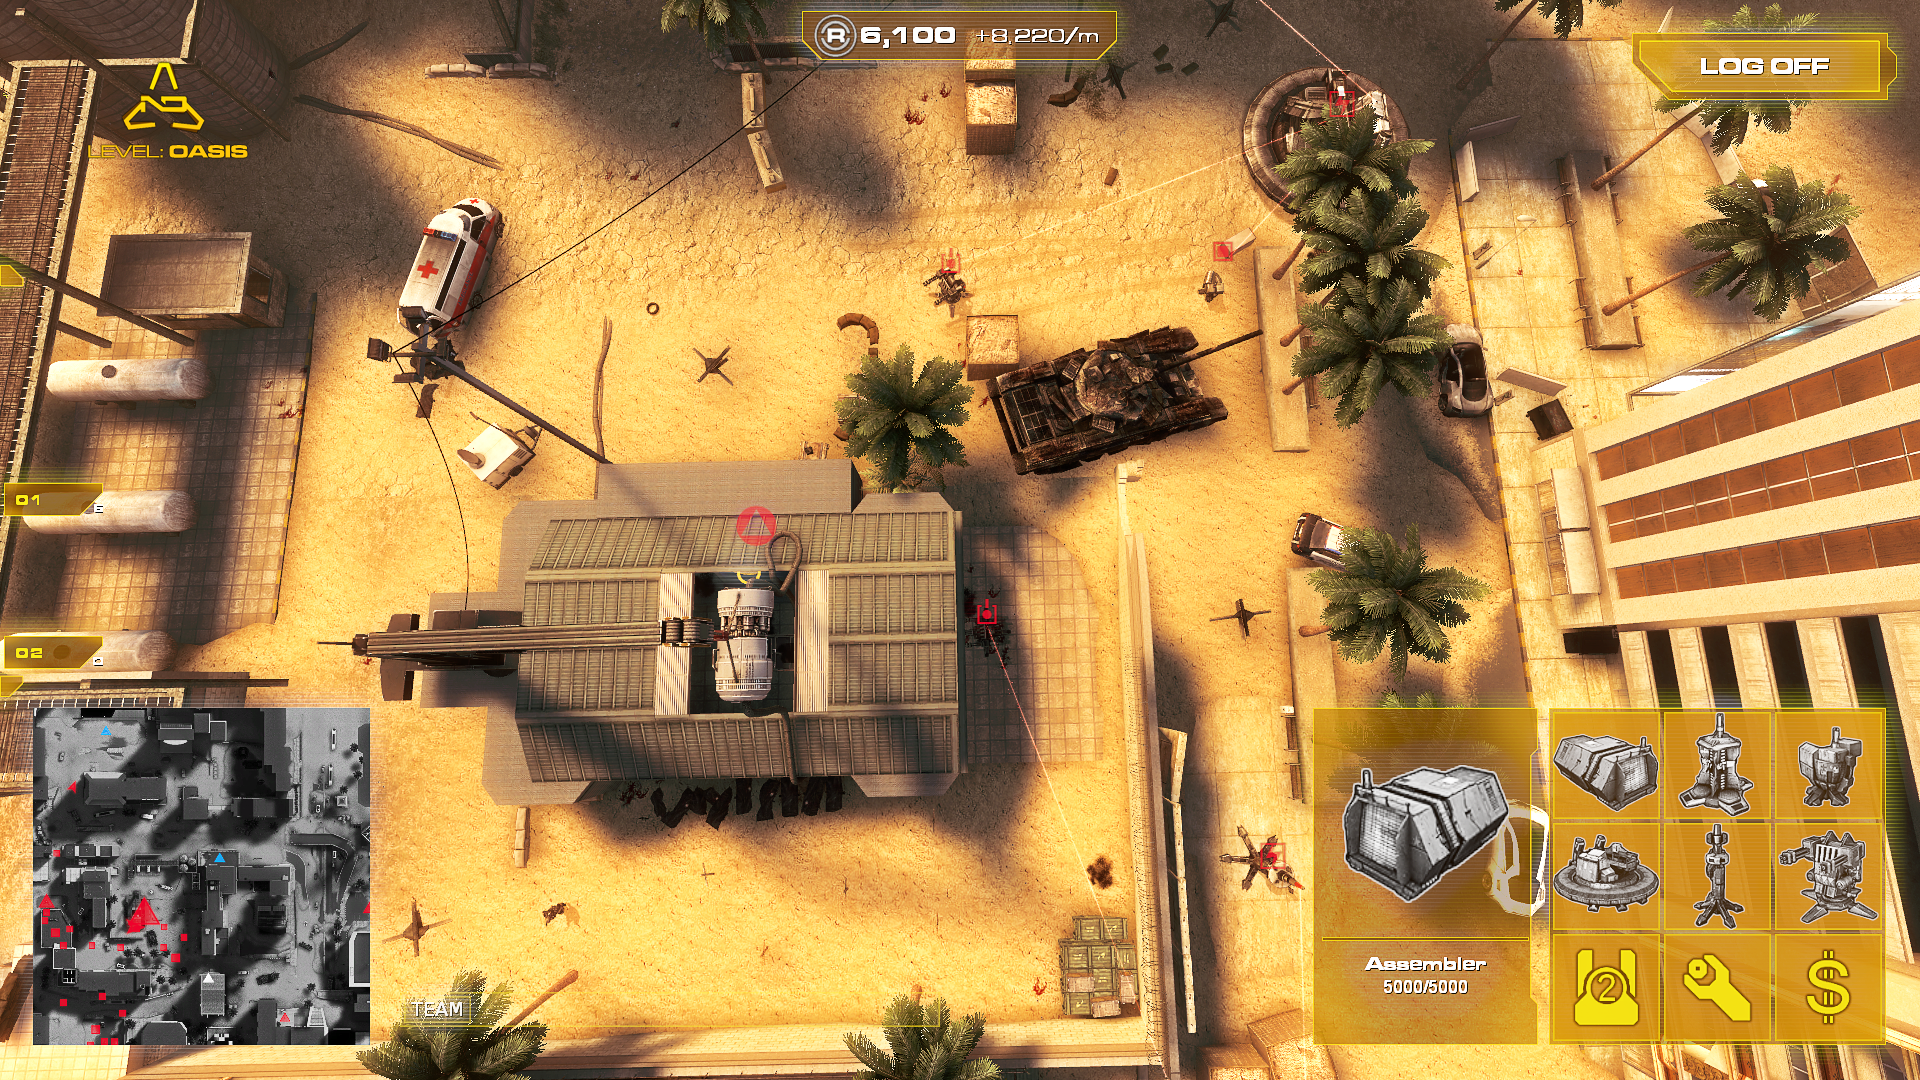
\includegraphics[width=\linewidth]{Nuclear_Dawn_-_Oasis_RTS_02.png}
	\caption{Typical top-down RTS view from the game Nuclear Dawn, by Interwave Studios. The view is of a courtyard and buildings, showing units (highlighted in red), a picture-in-picture map of the larger area (grey box in lower left corner), and game controls (yellow boxes in lower right corner)\citep{nucleardawn}.}
	\label{fig:Nuclear_dawn_rts}
\end{figure}

Realtime strategy games generally have the player playing against multiple other players, some or all of which may be controlled by the computer. 
The goal of the game is typically to acquire some form of resources, which are used to develop military units or units which accelerate the acquisition of further resources. 
The military units are then used to attack the other players, with the goal of the game being to be the only remaining player. 
Turn-based strategy games are similar to RTSs, but instead of all players acting simultaneously and asynchronously, each player's actions are taken on their turn. 

MOBAs have a smaller focus and more rapid play than RTS or turn-based strategy games. 
Typically, there are multiple players, but each player is on one of two sides battling over some set of objectives on the world map. 
Rather than controlling multiple units, each player controls a single, powerful unit, and may be able to influence weaker, semi-autonomous computer-controlled units.  There may be resources as in RTS games, but typically they are far more limited in number, as the emphasis of the gameplay is on action rather than resource extraction.   

MOBAs, RTSs, and turn-based strategy games all have a similar user interface. 
The ``world'' or area of play is depicted as a map, typically viewed either top-down or an axonometric perspective. 
The map is where the main action of the game takes place, and displays the relative position of the characters and other elements of the game. 
Around the map are typically displays and interactive elements such as menus or buttons to interact with the game. 

The control of units in the game is done using the mouse to select units and send commands via mouse clicks, while one hand operates keys, usually on the left side of the keyboard, for other functions. 
The use of the left side of the keyboard is to leave the right hand free to remain on the mouse, but these controls can be customized for left-handed players. 
How the keyboard is mapped depends on the pace of gameplay. 
For extremely rapid games, such as Defense of the Ancients (DoTA, a MOBA), there are a small number of key commands that can all be operated without removing the fingers of the left hand from the keyboard. 
DotA in particular uses mouse clicking, combined with the control, shift, and alt keys in various combinations, to perform all of the actions of gameplay \citep{DOTAControls}.

Age of Empires is a RTS. 
It is less fast-paced than DotA, but still takes place in realtime. 
Most of the keys of the keyboard are mapped to various commands, such as locating and selecting different types of units or buildings, or commanding those units and buildings. 
Commands to buildings typically cause the construction of various units, while consuming resources. 
For example, pressing `D' would find a Dock, and then pressing `A' would command the Dock to start work on a Fishing boat \citep{AOEControls}

Europa Universalis 4 uses the entire top row of letters on the keyboard to switch between different map modes, and every other key to activate some feature of the game, as well as mouse controls for interactions with individual units and locations \citep{EUControls}. 
Europa Universalis gameplay does not take place in realtime, and the player may speed or slow the game clock, as well as pausing the game. 

Another common feature of MOBA, RTS, and turn-based strategy games is the ``fog of war". 
The entire map is normally hidden from the player until they command their units to enter an area, whereupon the area is revealed. 
In gameplay, the intent of fog of war is to prevent players from knowing about the opposing player's location without sending sorties. 
This lack of information is almost identical to that experienced by a teleoperator of a robot exploring an area with a SLAM algorithm, with the map being revealed to the operator as the robot moves into the area. 

\subsection{Intel Drone Swarm Interface} \label{section:Intel_Drone_Swarm_Interface}

Intel has fielded drone fleets of up to 1,200 Shooting Star UAVs \citep{IntelDronesPage}. 
While the control system for the drones is proprietary, some information about the user interface can be gleaned from the promotional videos for the controller. 
The user interface for the creation of the light show appears to be very similar to those used in 3D rendering of computer graphics, including a timeline across the bottom of the screen, a preview in the center, and toolbars along the top and sides for interaction with the show. 
Visible tabs on the interface include "Curves/Surfaces", "Poly Modeling", "Sculpting", "Rigging", "Animation", "FX", "FX Caching", and "HEALTH". 
These different tabs are likely different ways to configure the shape of the formation in 3D (Curves, Poly Modeling, and Sculpting), animating the resulting formation (Rigging, Animation, and FX), and determining the state of the swarm as a whole (HEALTH). 

A screen that is likely part of the health interface is shown in one video \citep{OlympicTech}.
The screen has a grid of circles, colored various intensities of green, yellow, and red, as well as one shade of gray. 
The intensity may convey a different quality about the drone than the color, allowing at least two different dimensions of data per circle. 
As all the circles are displayed in a grid, an overview of the swarm health can be obtained by glancing at the display and assessing the relative balance of green vs. red. 

The user interface can import some form of data about the landscape where the drones will be launched, so the show can be positioned relative to hills or other obstacles in the area. 
The interface also supports at least some level of touch interaction, as users are shown pressing UI element buttons and rotating 3D renderings in the promotional videos. 

The interface for the drone light shows allows single users to fly hundreds to over a thousand drones, but it appears to be designed to create the show in advance, and execute it under central control. 
Overall, the interface seems to borrow from both interface design for 3D CAD, with animation elements and somewhat natural affordances for rotating and viewing 3D objects, and EID guidelines for presenting both high-level environmental information at the swarm scale, and individual unit health at the single drone scale. 
The readability of the health monitoring at a glance, by assessing the amount of green and red units is similar to the ambient monitoring available in Swarmish. 


\section{Swarm Software Development Methods} \label{section:Swarm_Software_Development_Methods}

Because the conversion of the specification of desired behavior for the swarm into individual programs for the swarm member robots is still an open question, it is necessary to understand the current methods used in the development of programs for swarm robots. 
Much of swarm robotic development follows the usual model of software development. 
Starting from a desired functionality, the developer writes a program that they think will provide that functionality.
The program is then tested, in simulation or on real robots, and its behavior is observed. 
The programmer then modifies their program to account for any observed difference between the desired function and the system's behavior. 
This loop of coding, testing, and coding again is repeated until the system behaves as expected, or the programmer graduates \citep{cham2010graduate}. 

Because the normal software development model is time-consuming, and outside of the abilities of many people who might want to use swarm robots, it is desirable to automate the development of software controllers for robots. 
One approach to the conversion of the command language to programs for the robots is to define a transformation from the command language to executable code. 
The transformation operation can be codified as a sort of ``compiler'', or more accurately, a code generator, which creates programs for the robots. 
The possibility of coding for the swarm as an entire system, rather than writing each robot's program independently, has given rise to several programming paradigms and domain-specific languages for robotic swarms. 

Another possibility is the composition of preexisting behaviors that each satisfy part of the user's desired behavior. 
Given some library of primitives, the user could select a sequence of behaviors, or conditions for the execution of behaviors, to build a complete program. 
Pheromone robotics provides one possible method of controlling this composition dynamically.
 
Still another approach is to allow the user to specify a desired behavior and evolving controllers to match it. 
It would be hoped that evolving the controllers would reduce the complexity of the development task to the definition of a suitable means of determining the fitness of the resulting program. 
Unfortunately, even this reduction does not permit an escape from iterative development. 

\subsection{Amorphous Computing} \label{section:Amorphous_Computing}

Amorphous computing (AC), also called spatial computing, is computation using locally-linked and interacting, asynchronous, unreliable computing elements dispersed on a surface or throughout a volume \citep{abelson2000amorphous}. 
The motivation for AC is that while it may be possible to produce arbitrary quantities of ``smart dust'', it is not possible to ensure that it all works well and is precisely located, especially in real-world applications.
The goal of AC is to get useful work out of such materials, despite uncertainty as to their reliability and location. 
Smart dusts are also the limit case, in terms of scale, for swarm robotics. 
Indeed, most of the volume of existing swarm robots is motors and batteries, with the computational components taking far less space. 
Unfortunately, the technology behind smart dust still does not exist, but programming methods for it have some applicability to larger swarm robots. \citep{Correll:2017:WRM:3131672.3131702}. 

There are several languages intended to program amorphous computers. 
``Proto" is a language for a continuous plane spatial computer which maps from behavior of regions at the global level to programs for discrete points at the level of individual devices \citep{beal2006infrastructure}. 
Because devices have a size in the real world, and space between them, the devices cannot not have a one-to-one mapping with the space, but instead perform an approximation of the desired behavior. 
Proto also has considerable appeal as a programming language for swarm control development because of the layering in its structure. 
If user interface interactions can be interpreted as indications of desired behaviors displayed over spatial regions, then conversion of those behaviors into programs in Proto may be amenable to automation. 
Proto's layered structure also has a clear relationship to the hierarchical structure of EID, with the programming language serving as a user interface at the highest abstraction level of the interface design, but providing a smooth transition to the lower abstraction levels.  

%Origami Shape Language (OSL) uses the abstraction of a foldable sheet to form shapes, inspired by both origami and the folding of epithelial cells during the development of biological organisms \citep{nagpal2004engineering, nagpal2001programmable}.
%Regions and edges on the sheet can be defined by propagation of morphogens, and folds along the edges result in the development of the final form.
%Because of the use of morphogens and local communication between the agents on the sheet, there is no need for a global controller to dictate the development of the final form. 
%Further, because the high-level description of the desired form does not involve abstractions of the underlying modules, OSL could operate on interlocking modular robots, actuated flexible materials, swarms, or other kinds of computational media. 
%In fact, the flexible sheet could be assumed to be virtual, and the resulting motions of the sheet could be translated into motor commands to configure swarm robots into specific arrangements in space. 
Growing Point Language (GPL) allows the specification of topological patterns in an amorphous computer, and so can also be used to specify the distribution of swarm robots, or behaviors of the swarm robots, in a space \citep{nagpal2004engineering}. 
GPL is inspired by the morphogenic controls present in biological organisms, which use gradients of chemicals called morphogens to dictate the development of cells \citep{turing1952chemical}.
The name GPL arises from one of the language's main abstractions, the growing point. 
The growing point is the location of activity within the amorphous medium, at which local agents are changing their state. 
Growing points move through the medium, affecting the state of the computational points they pass, and emitting pheromones into the medium which control the motion of growing points.

Importantly, GPL does not make any prior assumptions on the location of the particles in the system, or robots in the swarm, aside from that they are sufficiently dense in the medium. 
For swarm robotics, this is an important quality, as precise localization may not be available. 
Initially, all agents have the same state and program, with a few exceptions that serve as seeds for the growth to begin. 
If the pattern is not required to be fixed at a particular location, even the seeds could be undetermined initially, and elect themselves via a method such as lateral inhibition. 
During the execution of the GPL program, each agent chooses its state based on the presence of pheromones, which are morphogens with limited range. 
Range limitation on morphogens propagating between robots is set using a TTL (Time To Live) counter that propagates with the morphogen, and is decremented with each hop in the communication network. 
When the TTL hits zero, the morphogen message is no longer propagated. 
By controlling the production or propagation of morphogens within the amorphous medium, complex patterns can be developed. 

\subsection{Pheromone Approaches} \label{section:Pheromone_Approaches}

The abstractions of GPL bear a very strong relation to pheromone robotics. 
Pheromone robotics is a metaphor used in developing control software for swarm robots. 
Some social animals, especially insects, use chemical signals called pheromones to communicate with each other. 
For example, wasps inside their nest react to the scent of wasp venom by travelling to the outer surface of the nest and attacking nearby moving targets  \citep{jeanne1981alarm}.
Ants leave trails of pheromones for other ants to follow to food sources. 
Each individual ant's contribution to the trail can be modulated by the quality of the food source, which allows the reaction of the other ants to the trail to cause an emergent distribution of the foraging work force that favors higher-quality food sources \citep{sumpter2003nonlinearity}.
Because pheromones are chemicals with spatial locations, it would be possible to combine the use of pheromones with reaction diffusion equations to structure activity within a space or to converge to patterns of activity over time  \citep{turing1952chemical}. 
Assuming even diffusion of the robots in space, the global map of the pheromone concentrations can be represented over the network by the locally-computed concentrations computed by each robot.

In pheromone robotics, the pheromones are usually simulated or ``virtual'' pheromones, rather than real chemicals which are detected by chemical sensors (for an exception, see \citep{hayes2001swarm}). 
Each pheromone can have properties such as diffusion and evaporation rates that result in the pheromone spreading in space or gradually disappearing. 
For example, a robot may emit a pheromone which diffuses into the environment and evaporates quickly, so distance from the robot can be determined by the strength of the pheromone, and approaching or avoiding the robot may be accomplished by moving up or down the gradient of pheromone strength. 
If the swarm is engaged in a search, each searching robot may emit a ``search marker'' pheromone that lingers in the area after the robot leaves. 
Other robots, on entering the area, would detect the pheromone and know that searching this area again would be fruitless. 
If the object of the search can move, the marker pheromone could diminish as a function of time, so areas that have not been searched for a long time become unmarked and may be searched again. 
Once the target is found, the robot may stop and emit a ``discovery pheromone'', which diffuses into the environment, attracts other robots, and causes them to also emit a discovery pheromone. 
As a result, once any robot discovers the target, all of the robots quickly converge on its location. 

The addition of directional communication for the messages that convey virtual pheromone information allows easy determination of the direction of pheromone gradients \citep{payton2001pheromone}.
Rather than directly diffusing in the space as a chemical would, hop counts in the network of robots simulate diffusion. 
Because routes may be of different length, the message with the lowest hop count is assumed to be the truest indication of minimal distance within the network. 
Rather than modelling the world based on the incoming messages, the content of the pheromone messages and the network behavior as a whole serves as a model of the world, mapped 1:1 onto the real environment. 
While it is possible to build a set of behavioral primitives out of pheromone signaling and associated behaviors, controlling the swarm to perform a task with these primitives is still done by hand \citep{payton2003compound}.

In all of these examples, the sensing of the pheromones is assumed to be local to the robot, at least metaphorically. 
To actually maintain pheromones in the environment without robots being present to transmit them requires, again, a global representation of the task space which the robots can refer to when needed. 
However, if some degradation in performance is acceptable, the robots can maintain a shared tuple space that lists information such as pheromone gradients and share it through local connections \citep{pinciroli2016tuple}. 

Use of pheromones to guide swarm robots for simulated search and patrol tasks has been demonstrated, with the assumption that there is a central controller maintaining the concentration of pheromones on the map, and informing the swarm members \citep{coppin2012controlling}. 
In a real implementation, some robots could remain stationary and only act as transponders, computing and transmitting the local pheromone information for a given area \citep{hoff2010two}. 
Another possible approach to enable pheromones in space is to operate the robots in an area which is illuminated by a projector. 
The projector can then color the area with light that the robots can sense, and modulate the intensity of the light to indicate the intensity of the pheromone \citep{arvin2015cosvarphi,diaz2017human}. 
However, even if the robots are limited to only the pheromones they can directly perceive and emit at the present instant, some emergent behaviors are still possible. 


It has been demonstrated that a swarm can perform construction tasks using only local sensing and no communication \citep{wawerla2002collective, bowyer2000automated}.
However, the addition of communication between systems and memory of the state of the world will improve the efficiency of the system.
Pheromone approaches can guide the construction of objects, even if the individual swarm members have no memory and only local perception \citep{mason2003programming}. 
The agents engaged in the construction move at random, and take actions governed by their individual perception of environment at present time. 
The agents can release and react to pheromones in the environment, and so there is an implicit communication via stigmurgy, but no explicit agent-to-agent communication. 
The set of rules that govern the mapping of sensor precepts to actions must be such that no point in the construction of the building can be mistaken for another, as that could result in loops or skipping parts of the building sequence. 
The TERMES project created a compiler that translates desired final structures into rules to guide the construction of those structures by cooperating agents \citep{werfel2014designing}.

\subsection{Vector Fields} \label{section:Vector_Fields}
Both global vector fields and the global and local blending of vector fields in co-fields can be viewed as subsets of pheromone robotics that use a global spatial representation. 
The vector field represents the space the robots are operating in as a continuous vector field with the magnitude and direction of the vector at each point in the field controlled by some system of equations.
By altering the specification of the field, the user can change the actions of the robots within that field. 
One approach to a control UI for a remotely-located swarm is a multi-touch interface for specifying a vector field \citep{Kato:2009:MIC:1520340.1520500}.
Because the user interface design focuses on the vector field rather than individual robots, the same control interface can scale to an arbitrarily large collection of robots. 
Vector field paths can have loops, which do not exist in waypoint-based paths. 
Waypoint paths have explicit ends, unless an additional command is added to join beginning and ending points. 

Vector field paths have substantial limitations. 
Because the vectors are bound to a 2-D plane, the paths they create cannot cross each other. 
Instead, they flow together. 
A 2-D vector field is also not a useful metaphor for controlling UAVs.
The vector field could be possibly extended into three dimensions, to control UAVs as well as ground vehicles, but there would have to be some form of discontinuity in the field to prevent assignment of UAVs to ground vehicle paths and vice versa. 
The vector field can be viewed as an abstraction of pheromone control, or even implemented in terms of the presence or absence of virtual pheromones, but it has some limitations that pure pheromone control does not have.
For instance, pheromones permit the presence of multiple pheromones at one point, with multiple meanings, but the vector field has one value for each point. 
Attempting to solve this problem by proposing multiple fields raises the question of how to combine the influences of each field, and if a universal combination function applies at all points in the field, it raises the question of why they were not combined in a single field under that combination equation. 

The vector field is also not very intuitive to users. 
Kato \emph{et al}. indicates that in order to use the vector field well, the users had to anticipate and project the future motions of the robots. 
Interface changes, such as showing particles on the vector field, could improve usability, but these approaches would have the same scaling problems that the robot representation does. 
When the view is zoomed out very far, individual whirls and eddies in the field may not be visible to the user. 

This vector field interface does not directly map to programs on the robots. 
Instead, the central computer maintains the vector field representation and commands the individual robots.
Vector fields also do not allow the assignment of tasks to robots, but allows the user to directly control the motion of the robots. 
In order to convert from a task-based user interface to a vector field representation, the task would have to be converted into a series of changes to the field.
Since the robots may not have accurate localization within the task space, it may not be possible to guide the robots by relating their position to a global vector field. 

The use of co-fields may provide a way to move the vector field representation from the central computer to the swarm, or allow the swarm to act for some time without constant updates from a central controller \citep{mamei2003co}.
Co-fields distribute the data within a space, which may be physical or may be abstract. 
Agents react to gradients in field, and spread their own fields over local communication networks. 
The overall vector space created by the user (the UI vector space) could be propagated to the robots periodically, and combined with their own internal vector fields to generate movement based on both the user's desires and the local rules operating on each robot. 
As with general vector fields, knowing which areas of the UI vector space are relevant to each robot may require global localization, and so only be available for swarms operating in conditions that permit global localization. 

\subsection{Compositional Approaches} \label{section:Compositional_Approaches}

Rather than developing a novel control program for each robot automatically, it may be possible to compose programs from behavioral primitives, such that some combination of the primitives results in the emergence of the desired behavior. 
A compositional approach to program generation requires the definition of primitives out of which programs can be composed, and some degree of assurance that these primitives can cover the space of possible tasks required from the robot. 
One possible list of primitives is disperse (no other nodes within distance d), general disperse (no more than n nodes within distance d), clump/cluster, attract to location, swarm in a direction, and scan area \citep{evans2000programming}.
Another proposed catalog of behaviors for swarm control bases the simple behaviors on pheromones or chemical sensing in single cells \citep{nagpal2004catalog}. 
The proposed behaviors are the use of gradient sensing for position and direction information, local inhibition and competition, lateral inhibition for spatial information, local monitoring, quorum sensing for timing and counting, checkpoint and consensus sensing, and random exploration. 
The first five are common in amorphous computing as well, but the last three are not. %TODO what are their uses?. 
While these behaviors are themselves expressed in terms of pheromones, the composition of the primitives into complete programs is not dictated by a pheromone-based system.
Furthermore, compositional approaches have been proposed in control-theoretic terms as well as pheromone-based terms, so the process of composition of primitives can be viewed as a metastrategy for the creation of programs, rather than a process specific to pheromone robotics \citep{belta2007symbolic}.

%The pheromone based approaches to swarm programming are sufficient for relatively complex behaviors. 
%Quorum sensing is used to detect whether the local agent count is sufficient for a task. 
%By detecting the presence of sufficient robots to perform a task, the robots can allocate themselves to tasks in a just-in-time manner, rather than being pre-allocated when the task is designed. 
%Decentralizing the selection of robots, in turn, may be more robust against failures of individual robots, as it uses the robots that are in the right place at the right time, rather than waiting for specially assigned robots. 
%However, under sufficiently bad conditions, a sufficient quorum may never arrive, deadlocking the task. 
%In combination with domino timing, where completion of each phase triggers the next, locking at any step could then deadlock the entire process unless another mechanism detects and corrects it.

%This stuff not actually compositional

%Individual robots can cooperate without communication to push an object to a beacon based on simple behaviors \citep{chen2015occlusion}. 
%Each robot has two simple behaviors.
%If the view of the beacon is blocked, and the robot is next to an object, the robot pushes on the object.
%If the robot can see the beacon, it wanders and avoids obstacles. 
%The sum of the two behaviors results in a net pushing force on the side of the object opposite the beacon, which moves the object to the beacon. 
%There do exist certain pathological shapes which the system cannot move towards the beacon, but it is demonstrated to work for all convex shapes. 

Another compositional method for programming robots proposes that the behaviors can be separated into classes, such as motion, orientation, and so forth \citep{mclurkin2004stupid}. 
Among these behaviors are ``primitives'' such as several forms of clustering, which other, later works have treated as an emergent behavior itself, arising from more primitive primitives. 
The variable granularity of the primitives available to compose swarm control programs seems to point to a hierarchy of control elements, with perhaps single motor operations at the bottom, and an increasing composition of elements to create more and more complex behaviors.
Swarm control programs would then call multiple primitive behaviors, providing them with parameters such as degrees of bearing and centimeters of proximity. 
The behaviors ideally run concurrently, and some of them respond to sensor inputs. 
The output of behaviors is whether they are running, translational and rotational velocity for the robot, and LED configuration. 
Because multiple behaviors might specify differing outputs, subsumption and summation are used to arbitrate between behaviors of differing priorities. 

These emergent approaches do not have the robots perform all of their available actions all of the time. 
Instead, it is assumed that the behavior of each robot is controlled by its reaction to the environment around it, and possibly to signals from other robots, so that actions are only performed when they are required. 
As a result, user programs compiled from a higher-level representation could be a table consisting of possible values for the sensors, and the actions to undertake when those values are met.
Guarded Command Programming with Rates (GCPR) provides a formal framework for the analysis of this type of compositional program \citep{napp2011compositional}. 
Robots are assumed to only have local sensing.
The guards of GCPR are conditions on the environment.
When a condition is met, the robot performs actions at a given rate. 
In the concurrent case, this is modeled as each action happening one at a time, but in random order. 
On a real swarm, the actions would take place in parallel, but the concurrent model is more amenable to analysis. 
To determine if a set of actions will be successful, it is required to ensure that for all orderings of all actions, the final state space of the swarm is the desired final state. 
Correct programs are those that reach the target state with probability one, even when composed with bounded failures. 
Once the target state is reached, the program is assumed to halt, so while the final state may be reached very slowly, once it is reached, it is not left. 
In the GCPR models, the time to execution of an action is stochastic, but in the real-world case of noisy or imperfect sensors, the variable time to execution of a guarded behavior would be caused by the imperfection of the robot's ability to detect that the guard was satisfied. 

\subsection{Evolutionary Composition} \label{section:Evolutionary_Composition}

Determining how the behaviors should be composed for an individual swarm robot's controller is difficult. 
Unfortunately, much of the process of composing of programs for swarm robots consists of iterating between composing sets of primitives and observing behavior of the system in an ad hoc process, just as with the creation of control programs by coding \citep{palmer2005behavioral}. 
Rather than removing iterative software design from the process, it has simply been moved up one layer of abstraction, from writing code for the robots to composing that code from behavior primitives. 

One possibility is to permit composition to behave like the programming environment Tierra \citep{ray1991approach}.
In Tierra, there is no such thing as an invalid program. 
All sequences of the existent symbols are regarded as executable programs, although some are more useful than others. 
The possibility that programs can be ranked by some function creates the possibility that genetic algorithms (GA) can direct the automated composition of behavioral primitives into programs \citep{palmer2005emergence}.
A GA expresses the robot program as a genome, which is translated into the actual program and run on the robot. 
The result of running each program is assessed using a fitness function and then the genomes for the best programs are combined to produce a new generation of genomes. 
This cycle of combining and assessing genomes continues until a certain level of quality is reached, as judged by the fitness function.

Unfortunately, given the time required to iterate over multiple generations of controllers, genetic approaches are unlikely to be fast enough for interactive control of robots by a human user. 
However, it is still useful to examine the possibility of developing a fitness function as a way of investigating methods for automatically assessing the behavior of a swarm.
Without some way of determining the ``goodness'' of a swarm's behavior, it is difficult to say that one algorithm or design paradigm is better or worse than another. 

In order to determine the quality of the behavior of the swarm, its behavior must be measured.
Harriott \emph{et al}. propose that metrics for measuring the interaction of humans and swarms differs significantly from the interaction of humans and individual robots, and can be broken down into 9 classes \citep{harriott2014biologically}. 
\begin{itemize}[noitemsep]
\item Human attributes - Interaction, trust, intervention frequency 
\item Task performance - Ability to accomplish task, speed, accuracy, cost
\item Timing - Command diffusion lag, behavior convergence
\item Status - Battery life, number of functioning members, stragglers
\item Leadership - Interaction between special members of the swarm and others
\item Decisions - Action selection, likelihood that the correct action is chosen
\item Communication - Speed, range, network efficiency
\item Micromovements - Relative motion of individual swarm elements
\item Macromovement - Overall swarm motion, flocking, elongation, shape 
\end{itemize}

Task performance is an especially interesting metric, but it is difficult to automatically extract from the observed behavior of the system an overall understanding of the progress it is making on the task, and so a value for the output of the fitness function. 
Worse, without a time bound on solving a problem or a way to calculate progress, it is impossible to tell if a program has failed, or has merely not yet succeeded.
For example, assume a program's intended purpose is to gather all of the units of a resource at a goal. 
If the program merely moves the units stochastically, sometimes they will enter the goal, creating an appearance of progress. 
However, it may be vanishingly unlikely that all the units will randomly happen to be in the goal at once. 
Counting the units moved to the goal, then, cannot distinguish between a program that cannot find the goal, and so will never put any units in it, and a perfect resource-gathering program that just has not moved any units to the goal yet.
 
Ideally, it would be possible to recognize and evaluate performance on sub-problems. 
It has been proposed that the interactions and emergent behavior of the system are observable, while the reactions of the agents in the system are programmable, and so by observing the interactions and emergent behavior, the developer can receive feedback on how the system is progressing \citep{palmer2005behavioral}. 
However, all of the proposed observation and hierarchy of reaction and emergence is intended as a design process, not an automation process. 
In other words, while the observation and hierarchical structure may guide the development of an emergent system, the system is still developed by programmers writing code and then running it on the robots.

In the limit, the swarm could be treated as a gas, and for tasks such as diffusion over an area, the performance of the swarm would be compared to the behavior of an ideal gas \citep{jantz1997kinetics}.
The addition of sensors and computation would then allow the robots to outperform a gas at tasks, and so achieve higher scores on a task-oriented metric than a gas could attain. 
Unfortunately, this metric is constrained to tasks that an ideal gas could perform, which are largely restricted to diffusion and alteration of density in response to temperature. 

Controllers have been evolved to allow robots to move into formation from random starting positions \citep{quinn2003evolving}. 
These controllers use local interactions and minimal sensing to achieve their goals. 
One point the authors make, which is not frequently mentioned in other work, is that while flocking or shoaling behavior is a relatively simple behavior to have emerge from robots who can detect the distance, position, and velocity of the other nearby robots, implementing that perception on real robots is quite difficult.
Because a specific behavior was desired, the fitness function used to evolve it was specified in terms of metrics related to the behavior. 
Task-specific fitness functions are also found in later work on evolution of swarm robot behavior, which seems to indicate that evolution of behaviors in swarm robots may only be a time-complexity trade-off. 

Interestingly, some of the work in evolvable controllers leads to inter-robot communication as one of the emergent properties of the evolved controller \citep{quinn2001evolving}.
In order to move as a formation, one of the robots must be the leader, but there is nothing in the fitness function or any of the other code that designates roles for the robots. 
Instead, the selection of the leader arises from the evolutionary development of the controllers, and is present in the controller as a response to a particular series of stimuli. 
Genomes that did not encode such a symmetry-breaking reaction never developed a leader-follower distinction, and so failed to move in formation, and so received low fitness scores. 
For the follow-the-leader task, genetic variation among the robots increased fitness more readily than having all robots share the same genome \citep{quinn2001comparison}.
The condition where all robots shared the same genes was called ``clonal", while each robot having its own genome was ``aclonal".
Oddly, while one would expect that the aclonal condition would result in a specialization, with each robot developing a genome that performed either the leader or follower role well, the aclonal condition developed robots which could perform both roles. 
It was hypothesized that while the clonal condition had to evolve roles and an allocation mechanism simultaneously, the aclonal condition could specialize the roles during early evolution, and then develop an arbitration mechanism to select roles.

Genetic algorithims have also been used to develop aggregation behavior in swarm robots \citep{bahgecci2005evolving, dorigo2004evolving}.  
Aggregation was chosen because it is a preliminary behavior primitive, which the swarm might engage in prior to doing some other task, such as moving an object or attacking together.
The resulting controllers only controls aggregation behavior, so each behavioral primitive would require its own evolutionary development. 
Solutions discovered by genetic algorithms are also prone to overfitting. 
The swarms described in Dorigo \emph{et al}. decreased in performance when the number of robots involved in the swarm was changed from the values used to evolve the solutions, and when a more accurate physical model was used in the simulations.

An interesting recent application of genetic algorithms (as well as simple exhaustive parameter searches) it the development of swarm robots that operate without computation. 
These robots are generally theoretical, rather than actually implemented in hardware. 
They typically have one sensor, which is binary and detects the presence or absence of an obstacle, and a program consisting of an if statement that branches according to the output of the sensor. 
The output of the program is typically the speed of two wheels in a differential drive arrangement.
Despite the minimalism of the model, by tuning the output parameters of the robot, they can be configured to form stable circles, and with a few more sensor states, to aggregate, shepherd ``sheep'' robots, forage, gather objects, follow walls, and disperse \citep{gauci2014self, johnson2016evolving, ozdemir2017shepherding, brown2018discovery, stcircle}. 

While these abilities of computationless robots actually do cover the desired tasks from the user experiment in chapter \ref{chapter:user_experiment}, this approach has some problems with transition to deployment on real robots, rather than point robots in simulation. 
The simulations used in computationless swarming frequently assume a perfect sensor of infinite range, which is unlikely to exist on a real robot.
However, at least one study was performed with sensor noise that could change the sensor reading, causing it to indicate incorrectly with probability $p$, and found that the controller outperformed doing nothing, so long as $p$ was less than 0.5 \citep{gauci2014self}. 
While extensions which admit a sensor that can detect obstacles, and so avoid it, are no doubt possible, there are more troubling results that indicate that the general design problem for an computation free swarm in an arbitrary environment is NP-complete \citep{wareham2018viable}
Further, the use of evolutionary programs is still prone to long run times for the evolutionary algorithm itself, and to exploiting errors in the statement of the fitness function. 
As a consequence, it is ill-suited to user interaction with users who are not experienced in genetic algorithms. 

The common hope of users of genetic algorithms is that they can reduce the complexity of directly specifying the task to the (hopefully lower) complexity of describing the results in the fitness function.
Rather than describing how to solve a problem, one simply describes what the solution would look like. 
Unfortunately, the reduction in hands-on time spent programming frequently comes at the expense of time spent waiting for the system to converge, or determining why it converged on a problematic solution. 
One attempt to evolve aggregation controllers had a fitness function which allowed the evolved motion strategy to acquire a high fitness by spinning in place.
The ad hoc iterative process of creating emergent behaviors is replaced by an ad hoc iterative process of creating fitness functions.
As a result, developing novel behavior in the field by converting user specifications of the behavior of the swarm into a fitness function for a genetic algorithm is unlikely to yield results in a timely manner. 
However, individually evolved primitives could be saved in a library of primitives for use by a higher-level compositional approach. 
Such a library could take advantage of the possible overfitting of GA evolution by storing primitives intentionally overfitted to specific situations and robots, and using the best matches. 
For example, a controller that aggregates small-scale UAVs outdoors is likely quite different from one that aggregates medium-scale wheeled robots indoors, even though they are both aggregation controllers. 

\subsection{Domain-Specific Languages for Swarms} \label{section:Domain_Specific_Languages_for_Swarms}

Proto and other programming languages for amorphous computers provide abstractions for computation performed on homogeneous spatially-distributed computing nodes, but do not generally support motion of nodes within the space. 
Other versions of tuple-space based amorphous computation include motion of the agents, but do not explicitly support heterogeneity \citep{viroli2012linda}.

The Voltron programming language provides what its authors describe as ``team-level programming'' for autonomous drones \citep{mottola2014team}.
This level of programming is distinct from drone-level programming, where specific instructions are provided to each drone, and swarm programming, where each drone has the same instructions and operates without communication with other drones.
Voltron programs consist of sensing tasks that are subject to space and time constraints, so the language does not permit the user to specify direct interactions between drones. 
This leaves out activities beyond sensing that may be useful for swarm robots, such as patrolling an area or collaboratively moving an object.
Additionally, Voltron is based on the assumptions that drones have global localization, synchronous clocks, and reliable inter-unit communication.   

Karma provides a programming framework for micro-aerial vehicles with minimal localization and no communication in the field \citep{dantu2011programming}.
The framework allows the composition of behaviors described at the level of individual robots. 
Rather than each robot performing a set of behaviors in response to input from its sensors, each robot is tasked by a central ``hive'' to perform a single behavior, such as performing a sensor sweep of an area. 
The hive collects data from robots as they return to the hive, and updates a central data store, which includes both the sensor information from the individual robots and spatial information about the sensor information. 
The hive then assigns activities to robots based on rules that use the central data store to determine which activities should be performed. 
As a result, while the individual robots are autonomous and not in communication with the hive while operating, the hive maintains a central data store that is used to guide the future behaviors of the swarm. 
This model does permit a form of interaction between swarm members, in that information from one swarm member can inform the behavior of another member, but it does not permit dynamic collaboration between swarm members while they are operating away from the hive. 

Meld is a programming language for robot ensembles, which are composed of individual modular robots \citep{ashley2007meld}. 
However, many of the problems facing an ensemble of modules are the same as those facing a swarm, such as determining the overall goal, moving to proper positions, and detecting when the goal has been acheived. 
Meld is written in terms of facts and rules. 
Facts describe things such as adjacency between robots and location of robots. 
Rules are applied to facts, resulting in the generation of new facts. 
By including rules that generate facts which describe motor actions, the application of rules to the known state of the system can create a ``to-do list'' of actions for individual members of the system to perform. 
Rules are said to ``prove'' facts, and when no further facts can be proven, the system has arrived in a final state. 
Since facts that alter the state of the world can make previous facts false, the set of facts available must be periodically purged of facts that no longer hold. 
The authors of Meld point out that logic programming, of which Meld is an example, is poor at representing state beyond what can be computed as a consequence of the base facts. 
However, it is also claimed that the use of aggregates, which compute results based on the provable facts, can be used to store state about the system, avoiding this restriction. 

Buzz is a programming language and a virtual machine (VM) to run it on that is designed for programming swarm robots \citep{PinciroliLB15}. 
Each robot is assumed to be running the same bytecode on the Buzz VM (BVM). 
Buzz is also based on the assumption that robots exchange information in a situated manner, with any robot that receives a communication also being able to estimate the relative location of the source of that communication.
In order to support programming for swarms, Buzz treats the swarm and virtual stigmergy as first-class objects in the language. 
Swarms in Buzz provide an abstraction for a group of robots that allows the programmer to have every robot in the group execute a function, as well as dynamically create and disband groups. 
Virtual stigmergy provides a global, distributed data store for the swarm. 
The implementation of the virtual stigmergy structure allows the robots to maintain relatively up-to-date versions of the values stored in the data store, and to refresh them after recovering from failures of network connectivity.
Buzz also provides a convenient abstraction of the neighbours of the robot executing the program, which usually consists of all robots within communication range. 
Using the neighbours abstraction, the robot can, for instance, query all its neighbours about the value of a sensor precept at their location, in order to build a local map of the intensity of the sensed quantity. 

%A Minimalist Flocking Algorithm for Swarm Robots
%Christoph Moeslinger, Thomas Schmickl, and Karl Crailsheim
%	Simulated flocking 
%	Can work with heterogeneous robots as long as they use the same sensing method (IR rangers)
%		Doesn't actually justify how they know this, though
%		Robots heading/motion is abstract, so could be mobility-heterogeneous
%
%Self-Organized Flocking with a Heterogeneous Mobile Robot Swarm
%Alessandro Stranieri, Vito Trianni, Eliseo Ferrante, Carlo Pinciroli, Marco Dorigo, Ali Emre Turgut, Mauro Birattari
%	Heterogeneous
%	Aligning robots can agree on a common heading
%	non-aligning robots cannot
%	Behavioral heterogeneity
%	Boids - seperate, cohere, align
%		This work, some robots don't align
%	As proportion of aligning robots drops, performance degrades
%
%Mixed Species Flocking for Heterogeneous Robotic Swarms
%Sifat Momen, Bala P. Amavasai, Nazmul H. Siddique 
%	Defines flocking efficiency as percentage mean number of agents participating in a flock
%	Two types of agents, can tell each other apart
%	Variable heterospecific attraction (tendency to join each other's flocks)
%		Increasing this increases efficency
%	Doesn't really indicate why heterogeneity is cool
%		Birds apparently form mixed flocks for predator defence
%
%Flocking for Heterogeneous Robot Swarms: A Military Convoy Scenario
%Christopher JR. McCook and Joel M. Esposito
%	2 unit types, supply unit and defender unit
%	Control based on potential field derived from stated goals of the units
%
%Swarmanoid: A Novel Concept for the Study of Heterogeneous Robotic Swarms
%By Marco Dorigo, Dario Floreano, Luca Maria Gambardella, Francesco Mondada, Stefano Nolfi, Tarek Baaboura, Mauro Birattari, Michael Bonani, Manuele Brambilla, Arne Brutschy, Daniel Burnier, Alexandre Campo, Anders Lyhne Christensen, Antal Decugnière, Gianni Di Caro, Frederick Ducatelle, Eliseo Ferrante, Alexander Förster, Jerome Guzzi, Valentin Longchamp, Stéphane Magnenat, Javier Martinez Gonzales, Nithin Mathews,
%Marco Montes de Oca, Rehan O’Grady, Carlo Pinciroli, Giovanni Pini, Philippe Rétornaz, James Roberts, Valerio Sperati, Timothy Stirling, Alessandro Stranieri, Thomas Stützle, Vito Trianni, Elio Tuci, Ali Emre Turgut, and Florian Vaussard
%(37 authors, but it was a big project...)
%	Accuses swarm systems of being homogeneous as an oversimpification of natural systems, e.g. all worker ants
%	Footbots (wheeled, with omnicams)
%	Handbots (climbers and manipulators)
%	Eyebots (flyers, with cameras for overhead views)
%	No centralized control
%	Swarm + Humanoid, intended to refute the idea humans are the best form to operate in human-designed spaces
%	Interchangalbe parts, gives robustness
%	Local ad-hoc groups and structures to perform tasks
%	Being able to physically interact adds complexity to design
%		Manipulation and sensing methods must be compatible to allow interaction and communication
%		Robots may have very different perceptions and want to communicate about them
%	Indirect relationship between what individual robot is doing and what swarm as a whole is doing
%		Heterogenieity increases complexity
%	All the robots do IR comms and range/bearing sensing
%	Eyebots collaborate to localize off each other
%		Other robots can also localize off of them

\subsection{Program Generation from Formal Specification} \label{section:Program_Generation}

Controllers for modular robots that allow them to form shapes under stochastic mixing have been automatically generated from descriptions of the desired shape \citep{klavins2002automatic}. 
These controllers are focused on structures and formations that can be expressed as a tree. 
They do not relate the structure to any other point in space, but are purely in terms of connectivity between modules. 

Other work with modular robots has used sensing to characterize the environment and decide on the reconfiguration of the robot that will best allow it to complete the assigned task \citep{daudelin2017integrated, jing2016end}.
The high-level planner uses linear temporal logic in a tool called LTLMoP (Linear Temporal Logic MissiOn Planning) to synthesize a controller for the robot task, and from the behaviors required from the controller, a sequence of transformations of the robot into forms that provide those behaviors. 
	
Generation of programs from e.g. LTL descriptions of the task and environment are promising because they can generate provably correct controllers.
Unfortunately, these approaches to program generation are prone to extreme conservatism in the face of an unknown environment. 
Assume that a robot is placed in a simply-connected maze, with instructions to traverse the maze. 
Selecting one wall, either the left or the right, and following it, will result in the robot finding the exit, or returning to the entrance if there is none. 
However, the \emph{a priori} generation of a motion plan to reach the exit from the entrance is impossible, as the actual path taken is unknown. 
LTL and similar logics can only work on what is known about their environment, and so cannot operate in unknown environments. 
	
A potential method to extend LTL or other logics to an expanding environment is to develop what is known about the environment as the robot explores, and rebuild the controller as new facts are added. 
When the robot has explored enough, it will become possible to build a controller that achieves the desired result, or prove that it is not possible because the entire environment has been explored without gaining enough information to build the controller. 
While effective in theory, this approach can run aground on combinatorial problems, particularly in dynamic environments, as the facts may vary often, and require reworking of the controller. 

One approach to correct-by-construction controller synthesis for dynamic environments combines an offline LTL-based planner with an online motion planner for collision avoidance \citep{alonso2018reactive}. 
Rather than replanning as the environment changes, the system generates alternative plans, or explains to the user why no alternative plan satisfies the requirements.  
Unfortunately, this controller synthesizer still relies on a known map of the entire environment (but not of the obstacles in it). 
For real-world applications in disaster recovery, the map may not be available, or may be undergoing constant revision by the disaster. 
The synthesizer also creates revisions to the assumptions about the environment, and the number of these revisions grows combinatorially. 
Each revision is an assumption about the environment which must hold for the controller to be correct, such as "There will never be a deadlock if robot 1 is not in the hallway when robot 2 enters the hallway".
The revision can be viewed as a constraint on the motion of the robots, preventing robot 1 from entering the hallway, or robot 2 from entering the hallway if robot 1 is in it. 
With one robot in a fairly simple map, the paper indicates that 16 revisions are needed. 
Adding a second robot increases this to 1306 revisions.  

Combinatorial explosions are a frequent problem in synthesis of provably correct controllers. 
Mehta \emph{et al} presented work that that synthesizes not just the controller, but the entire robot \citep{mehta2018robot}.
In the controller, the sensors are represented by binary propositions of the controller logic, one for each possible sensed object.
For small cases, this is sufficient, but the number of such propositions is $2^{|objects|}$, and so becomes unwieldy for more complex specifications and robots.  
However, it does pose an interesting argument for heterogeneity of robots. 
Rather than changing how a swarm of robots with a fixed morphology is used to perform a task, robots can be generated as needed for tasks and added to the swarm. 
One would expect that once a diverse enough pool of robots exists, the work of Mehta \emph{et al} could be extended to select combinations of existing robots to perform a task, rather than creating new ones. 

%Translating Temporal Logic to Controller Specifications
%Georgios E. Fainekos, Savvas G. Loizou and George J. Pappas
%	LTL -> Hybrid automaton -> control spec
%	Control specification is probably for movement, continuious moves despite discrete states
%	Event-based semantics for LTL can't distingish events that must hold at an instant from those that must hold over a time period
%	Combines continuious flows (vector field) with discrete control transitions
%	I think this is making some assumptions of a pure holonomic robot on the ideal plane
%	
%From High-level Task Specification to Robot Operating System (ROS) Implementation
%Kai Weng Wong and Hadas Kress-Gazit
%	Automatically suggests possible fixes for mapping from controller to ROS
%	"While many of these approaches have been demonstrated on physical robots, the low-level integration of the provably-correct, typically symbolic, controller with the hardware is usually a manual and robot-specific ad-hoc process"
%		MURI integration 
%	Assumes single rosmaster, and no node launches another node as part of execution
%		Pretty reasonable
%	Talks about a boolean person detector
%		This stuff frequently gets really noisy, people can be hard to detect
%		Although hitting a person you fail to detect is provably correct, it's not great
%	Permits easy integration of provably correct controllers to ROS
%		Doesn't deal with the problems with provably correct controllers
%			Perfect information
%			Perfect sensors/actuators
%			
%Decentralized Control of Robotic Swarms from High-Level Temporal Logic Specifications
%Salar Moarref and Hadas Kress-Gazit
%	High level temporal logic to controllers for safe nav of area
%	Imperfect synchronization
%	Again with the known map
%	This paper assumes static and known environment, but the approach used doesn't rule out reaction to dynamic environment
It has been suggested that LTL is not the best formalism for the description of desired behavior for robot controllers \citep{belta2007symbolic}.
Belta \emph{et al} also raises some other problems with symbolic control and planning as a paradigm for robot control. 
Among others, they point out that the invariance of the dynamics of the robots to certain transformations, such as rotation around certain axes, permits symbolic control. 
However, as pointed out by Rodney Brooks in ``Artificial life and Real Robots'', environment conditions such as carpet nap can change dynamics of the robots in ways that break the symmetry of the dynamics about some axes \citep{brooks1992artificial}.
In addition, the symbolic methods still have problems with incomplete knowledge, and dynamic worlds (which imply incomplete knowledge, as things may change without being observed). 
While valuable for the strength of the assertions they can make about the generated controllers, symbolic and formal methods still require some level of reactive or heuristic buffering from the real world, to present them with the atomic actions and perfect sensors that their assertions rely on. 
%(Hadas http://link.springer.com/chapter/10.1007/978-3-642-22110-1_54#page-1 makes a distinction between unsatisfyable and unrealizable specifications. Unsatisfyable specs are those that the robot cannot do in any environment. Unrealizable specifications are those cases where there exist environments that can thwart the robot. In Hadas' work, there's also the idea that environments are finite in number. )
%\unsure{``Best effort", based on the information available, it's worth an attempt vs. not worth an attempt.}
%\unsure{So since we can't tell if a program will succeed, and determining if it is impossible might not be tractable, how do we know if we've written a compiler that does this?}

Another potential approach to the generation of robot programs for swarms is the use of Supervisory Control Theory (SCT) \citep{lopes2016supervisory}.
SCT provides a method to formally synthesize controllers called ``supervisors''. 
Both the possible state transitions of the robot and the control specification are represented as state transition diagrams, and realized as generators. 
The generators are then composed into a synchronous automaton, which is the supervisor. 
Changes in state are caused by events.
Uncontrollable events are produced by feedback, such as from sensors or timers, and controllable events are produced by the supervisor to control the robot. 
The resulting controllers can be demonstrated to not deadlock, and with probabalistic extension into pSCT, also not to livelock, while safety can be formally determined by ensuring that there exists no path in the supervisor leading to a forbidden state \citep{lopes2017probabilistic}. 

However, SCT alone is not sufficient to automate the generation of robot programs.
The expression of the abilities of the robot and the desired behavior, as state transitions in some form, is left as an exercise for the swarm developer. 
SCT supplies a way of ensuring that the resulting program does what the specification requires. 
As noted in \citep{lopes2017probabilistic}, a specification which is logically incorrect, such as including a possiblity to livelock, will generate a program that can be formally demonstrated to match that specification, and so includes the specification's errors. 

EvoStick and AutoMoDe-Vanilla both provide automatic design of swarm robot software using a test-and refine method \citep{francesca2014experiment}. 
AutoMoDe creates controllers by combining parameterized modules in a PFSM. 
AutoMoDe-Vanilla outperformed EvoStick, which is a typical neural network control evolution algorithm.
It was also able to outperform unconstrained human programmers, but not humans using the same set of modules available to AutoMoDe. 
An enhanced ``flavor'' of AutoMoDe, AutoMoDe-Chocolate, outperformed even the constrained humans \citep{francesca2015automode}. 
The goal of using pre-defined modules is actually to simplify the design space, under the theory approaches such as evolutionary design of neural network controllers have, essentially, sufficient representational power to overfit to their test environment \citep{birattari2016observing}.

\section{Group Perception of Humans} \label{section:Group_Perception_of_Humans}

Because it is desirable to have the users operate in a manner that scales with the size of the swarm, and that because scaling implies that they treat the swarm as a whole, rather than as individuals, discovery of the factors that result in perception of groups as a single entity rather than a collection of individuals is important.
One potential guide to when users will stop treating robots as individuals and begin treating them as a group is the numerical point that humans come to regard a collection of other humans as a collective, instead of individuals. 
Unfortunately, that point is quite complex to determine, because humans have vastly more complex social interaction with each other than they do with robots, and elements of that social interaction color how humans think of each other. 

In perceptual psychology, gestalt perception provides a number of heuristics or principles that can influence whether a set of objects is perceived as a group. 
\begin{description}
\item[Proximity principle]
Objects near each other are perceived as a group.

\item[Common fate principle] 
Objects that move together are perceived as a group.

\item[Similarity principle]
Objects that are visually similar are grouped together.
\end{description}	

There are various other principles, and the order in which they are assessed or their relative strengths are unclear, so it is difficult to determine how a complex scene will be parsed. 
However, these general guidelines do appear to influence how people perceive groups of other people. For example, all of the people in a line or a parade move together, and so are perceived as a group, separate from people around them moving in other directions.
It has been suggested that these principles may enhance the intelligibility of the behavior of robotic swarms \citep{nagavalli2018algorithms}. 

Humans also make some distinction between aggregates and groups \citep{wilder1978perceiving}.
Groups have a boundary, such as a common belief or goal, and sharing that element makes someone a member of the group or not. 
Aggregates are random sets of people, who may have nothing in common.
The people inside a church at a given time are likely a group, the people on the sidewalk outside are more likely an aggregate. 
This factor, combined with the gestalt common fate principle, may be useful for encouraging users to think of a swarm as a group. 
Since it can be made explicit to the user that the swarm shares common goals, and the swarm can move together, the user would come to regard it as a group, rather than a simple aggregate. 

Whether a set of people is perceived as a group is referred to as ``entitativity", which is to say, how much like a single entity they are perceived to be. 
Groups with high entitativity are expected to have a higher degree of unity and consistency within the group. 
The smaller a group is, the more similar its members are perceived to be, which seems to indicate that smaller groups would have higher entitativity \citep{stewart2003trust}. 

Entitativity isn't a binary classification, with groups being either entities or not. 
Rather, it is a spectrum, with groups such as families or organizations at the high entitativity end, and groups such as people in line at the bank on the low entitativity end. 
By surveys, some clusters of groups have been elucidated, such as intimacy groups (family and friends), task groups (co-workers, juries), social groups (gender, race, class), and loose associations (parade crowds, fans of a music genre) \citep{lickel2001elements}. 
In a situation familiar to computer scientists, the analysis of perception of group entitativity is prone to the curse of dimensionality: what counts as a group is highly variable along multiple axes \citep{lickel2000varieties}.  
Among the factors influencing it are differences in the perceiver (level of need to perceive a group, individualism or collectivism bias), contextual factors (group membership or opposition), and properties of the group itself (visual or behavioral similarity).
Minorities become higher in entitativity due possibly to the perception of them as figures distinct from a ``ground'', as in the gestalt figure/ground principle, or because stereotyping increases the perception of similarity within the group. 
The perception of similarity within the group may be in turn be related to the gestalt perception of similarity, and so visually-similar minorities would be expected to have a higher entitativity than visually dis-similar groups of people. 
	
Research in the influence of group size on effectiveness of persuasion reveals that the gestalt principle of similarity works on the level of information as well as visual similarity \cite{wilder1977perception}. 
When a person is confronted by a group attempting to influence them, increase in the size of the opposition beyond about 3-4 people has little effect. 
Rather than treating each person in the opposing group as contributing a bit of information that might sway the subject, and so a large group would contribute many bits, the entire group is lumped together and contributes one bit of information. 
The first person from the group who expresses their opposition may be viewed as a leader, but the rest can then be dismissed as followers, expressing an opinion no different from the leader's opinion. 

Unfortunately, the study of the entitativity of groups makes it clear that the factors that humans consider when deciding how strongly an association of other humans count as a group extend well beyond how many of people are in the group.
Human perception of groups has less to do with exact count of people, and far more to do with common cause, visible similarity, tasks, interpersonal relations, and so forth. 
One potential upper bound that is simply numeric is Dunbar's Number, a constraint on the understanding of a social network placed by neocortex size \citep{dunbar1992neocortex}. 
For humans, Dunbar's number is estimated to be around 150 individuals, and beyond that, people would be expected to begin chunking the people in their social network into hierarchies or groups in order to keep track of a reduced number of entities (e.g. one group called "co-workers" instead of every individual on the team). 

\section{Human/robot Teaming} \label{section:human_robot_teaming}

One area that may have interesting insights into control interfaces for heterogenous swarms is work on human/robot teams. 
Typically, human/robot teams involve robots working along side humans in a team, as peers or subordinates. 
As a result, the interface design is primarily for control of the robots, and the return of data to the humans, rather than in control of the team as a whole.
One attempt to unify the command and control of a human/robot team did so by expanding previous work, which had only commanded robots \citep{lopez2017unified}. 
The resulting interface allowed the end user to command robots and humans using the same command modalities, rather than specializing the command set based on the type of unit being commanded. 
In user tests, commanders of human teams, robot teams, and mixed teams had similar performance, and used similar control strategies.
The use of similar control strategies is surprising, because this includes direct, joystick-like control of human team members, which the researchers originally thought would be an unusual way to instruct a person to move. 
The users also mentioned that having an interface that reflects the generally superior mobility and perception of humans would be an improvement, so while the unspecialized interface did not appear to hinder users, it may have not taken full advantage of the team ability. 
By similar arguments, it could be that an interface for a heterogeneous swarm should support special operations for robots that can support them, rather than attempting to treat all robots the same in the interest of interface consistency. 

The multi-robot interface is also distinct from a swarm interface, although there is some overlap. 
A purely swarm-oriented interface would issue commands to groups of robots, and not have the ability to command single robots, under the assumption that tasks assigned through the interface were not possible for a single robot to complete. 
A pure multi-robot interface is designed to command multiple robots as individuals, with their own tasks. 
The interface described by Lopez, Kuczynski, and Yanco is somewhat in the overlap area, as it allows group selection and task assignment as well as individual command, both as ``groups'' of one, using similar command interactions to the group commands, and direct, joystick-like interaction. 
The interface described by Humphrey \emph{et al} is an interface at the multi-robot end of the spectrum, as it does not appear to provide any faculty for assigning a task to multiple robots at once.
It does, however, encourage the user to be aware of the functioning of all of the robots. 

In this work, the description of the user interface does not position the robotic swarm as a teammate. 
Robots can be team members with humans, but they can also be treated as remotely-operated tools. 
Teleoperation is a case of treating the robot as a remotely-operated tool. 
Rather than taking any initiative itself, the robot does as commanded, acting as the remote user's eyes and sometimes hands in the environment. 
Indeed, a teleoperated system should be invisible to the user, with the UI acting as the user's interface to the remote environment, rather than to the remote robot \citep{larochelle2011establishing}.
Examination of the work on robotic teammates lists some points about teammates that the swarm described in this work does not share.  

Teammates make decisions during task execution, while considering the impact of those decisions on their teammates \citep{shah2011improved}. 
The system described in this paper does not have any mechanism for the system to consider how its decisions will affect the human user. 
Some of the design decisions were made by with the impact on the human user in mind, but these decisions were made by the author, not the system. 

Teammates communicate progress and provide support  to each other. 
This communication can be explicit, or implicit, by doing things like placing completed components of the task where the other teammates can see them. 
The system described in this work can only be viewed as communicating implicitly, by having the swarm behavior attempt to match the user expectation. 

Being a team or not can be viewed as a spectrum, with robots taking the place of equal peers at one end and remotely-operated tools at the other end. 
Safeguards, such as safe-mode teleoperation, where the robot can act to prevent collisions, are on the spectrum, but more towards the remote tool end. 
Safeguards do not permit the robot to assume responsibility for a role or task, which is a component of team membership \citep{bruemmer2005shared}. 
Taking initiative combined with assuming responsibility is the basis of leadership, which, in a team of equal peers, can be distributed rather than centralized. 
The system in this paper has a central authority, the human user, who commands, but is not commanded by the system. 
Humans find it easier to delegate responsibility to more human-like robots than to non-human-like robots \citep{hinds2004whose}. 
This is in keeping with the spectrum of remote tools versus equal peers. 
A non-humanoid robot is easier to perceive as a tool, and a tool is not blamed if its user makes an error. 
The difference in perception of humanoid robots can also serve as a design guideline, indicating that non-human robots are to be preferred if the robots are likely to be unreliable, as the robot's form will encourage people to take more responsibility themselves instead of delegating it to the robot. 

On the spectrum between teammates and remotely operated tools, the swarm described in this work is solidly at the tool end of the spectrum. 
The user controls the swarm in a task-based manner, assigning it a job they want done and then allowing the system to operate, much like a computer-controlled metal-cutting mill.
The robots used are non-humanoid, both in their depiction on the user interface and their physical construction. 

